\documentclass[UTF8,a4paper,11pt,openany,fontset=fandol]{ctexbook}
\usepackage[a4paper,margin=23mm,headheight=15pt]{geometry}
\usepackage{amsmath,amssymb,bm,mathtools,booktabs,longtable,tabularx,array,graphicx}
\usepackage{enumitem,xcolor,fancyhdr,needspace}
\usepackage[numbers,sort&compress]{natbib}
\usepackage{float}
\usepackage{hyperref,bookmark}
\usepackage{tikz}
\usetikzlibrary{arrows.meta,positioning}
\setCJKmainfont{FandolSong-Regular.otf}[BoldFont=FandolSong-Bold.otf,ItalicFont=FandolKai-Regular.otf]
\setCJKsansfont{FandolHei-Regular.otf}[BoldFont=FandolHei-Bold.otf]
\setCJKmonofont{FandolFang-Regular.otf}
\setmainfont{texgyretermes-regular.otf}[BoldFont=texgyretermes-bold.otf,ItalicFont=texgyretermes-italic.otf,BoldItalicFont=texgyretermes-bolditalic.otf]\setsansfont{texgyreheros-regular.otf}[BoldFont=texgyreheros-bold.otf]
\definecolor{ink}{HTML}{193D55}
\ctexset{chapter={format=\sffamily\huge\bfseries\color{ink},beforeskip=0pt,afterskip=20pt},section={format=\sffamily\Large\bfseries\color{ink}},subsection={format=\sffamily\large\bfseries},subsubsection={format=\sffamily\normalsize\bfseries}}
\hypersetup{colorlinks=true,linkcolor=ink,citecolor=ink,urlcolor=ink,bookmarksnumbered=true,bookmarksdepth=2,pdftitle={Hall MHD与双流体磁重联：模型推导、数值方法与文献调研}}
\setlength{\emergencystretch}{4em}\setlength{\parskip}{3pt}\linespread{1.12}\raggedbottom
\setlist{nosep,leftmargin=2em}\setcounter{tocdepth}{1}\setcounter{secnumdepth}{2}
\pagestyle{fancy}\fancyhf{}\fancyhead[L]{\small\nouppercase{\leftmark}}\fancyfoot[C]{\thepage}
\newcommand{\vct}[1]{\bm{#1}}\newcommand{\dd}{\mathrm d}\newcommand{\VA}{V_{\!A}}\newcommand{\J}{\vct J}\newcommand{\B}{\vct B}\newcommand{\E}{\vct E}\newcommand{\vel}{\vct u}\newcommand{\grad}{\nabla}\newcommand{\R}{\mathcal R}
\newcommand{\note}[1]{\par\smallskip\noindent\textsf{\textbf{学习提示：}}#1\par\smallskip}
\newcommand{\assume}[1]{\par\smallskip\noindent\textsf{\textbf{假设与边界：}}#1\par\smallskip}
\newcolumntype{P}[1]{>{\raggedright\arraybackslash}p{#1}}
\numberwithin{equation}{chapter}

\let\cleardoublepage\clearpage

\tracinglostchars=3
\usetikzlibrary{calc,decorations.pathreplacing,shapes.geometric}
\newcommand{\worked}[1]{\par\medskip\noindent\textsf{\textbf{完整算例：#1}}\par\smallskip}
\newcommand{\Deta}{D_\eta}
\renewcommand{\theequation}{\thechapter.\arabic{equation}}

\hypersetup{pdftitle={撕裂模：从磁岛物理图像到理论推导与实验检验}}
\begin{document}\frontmatter
\begin{titlepage}
\vspace*{20mm}
{\sffamily\Large 磁场重联 · 研究生入门讲义\par}
\vspace{15mm}
{\sffamily\Huge\bfseries\color{ink}撕裂模\\[8pt]理论推导与实验检验\par}
\vspace{14mm}
{\Large 磁岛怎样产生，增长率怎样算，实验怎样看\par}
\vspace{12mm}
{\large 逐项线性化 · 内外层匹配 · 非线性增长 · 完整算例\par}
\vfill
编写日期：2026年11月16日。\\[8pt]
阅读前提：学过等离子体导论，了解Maxwell方程、洛伦兹力和流体基本概念。讲义从磁通函数与磁岛图像出发，逐步引入共振面、渐近匹配与实验诊断。\\[8pt]
配图由附带脚本绘制，分别标为解析结果或教学示意。实验结论对应原始论文及图号；本讲义未宣称运行完整本征求解、重联数值模拟或复现实验。
\end{titlepage}
\chapter*{怎样学习，而不被公式淹没}
第一遍读第1章、每章开头和所有图注，建立磁面、X点、O点、内层与外区的空间图像。第二遍依次读第2--4章：先把复指数的相位约定和线性化每一项弄清，再理解为什么要把一个问题拆成理想外区与非理想内层，最后亲自复核增长率的幂指数和数值系数。第三遍读第5--6章，把理论量对应到线圈电压、温度剖面、磁通重建和质子照相。

公式中的“等号”表示在写明的近似模型内的关系；“$\sim$”表示量级或渐近标度，不能从中读取精确系数。$a$是平衡电流片半厚，$\delta_*$是明确定义的线性内层尺度，$W$始终是磁岛全宽。增长率$\gamma$是磁通扰动的指数增长率，岛宽在线性阶段按$e^{\gamma t/2}$增长。这几个差别贯穿整本讲义。

四章理论构成一条连续推导链：磁通/涡量方程，Harris平衡，线性化，共振面，外区$\Delta'$，FKR常磁通匹配，大$\Delta'$支，Rutherford增长，以及长薄片的plasmoid标度。后两章解释三类实验并给出逐项代入的量级和诊断算例。专门的源记录保留原文版本、核对范围和证据边界；本次讲义整理不改动原调研库146篇全文核读计数。

伴随讲义Lecture-HallMHD解释双流体、Hall项、电子冻结破坏和闭合。两份讲义都独立可读，但采用不同常见坐标：本卷$x$横穿电流片，$y$沿片，$\B_\perp=\hat{\vct z}\times\nabla\psi$。比较时先对齐定义，不要直接照搬分量符号。
\setcounter{tocdepth}{1}\tableofcontents\listoffigures
\mainmatter
\chapter{先看见磁岛，再建立撕裂模的方程}\label{tm:foundations}
\section{本讲义到底要回答什么}
撕裂模（tearing mode）是\textbf{电流片的拓扑改变型不稳定性}：一个很小的磁通扰动，在某些平衡中会自行增长，使原来从一端延伸到另一端的磁面分裂为磁岛。这里的“自行”是相对于持续外部强迫而言；能量来自原平衡的磁场与电流分布。电阻打开原先被理想磁冻结禁止的演化通道，并不作为供能电池。

有三个问题必须分开。第一，给定平衡是否有允许增长的扰动？这是\emph{稳定性}。第二，扰动以多快的速度长大、磁岛多宽？这是\emph{增长率与非线性演化}。第三，整个系统每秒重联多少磁通？这是\emph{重联率}。一个正增长率不等于最终稳态重联率，观察到一个磁岛也不能单独反推出线性增长率。

我们从最可控的二维、不可压、电阻MHD问题出发，真正算完外区解、内区尺度与两者的匹配。经典来源是Furth、Killeen与Rosenbluth的电阻撕裂研究；现代写法也可逐式对照Fitzpatrick的作者讲义。\citep{TMFKR1963,TMFitzMatching} 后文再说明该模型与实验、Hall模型和动理学模型的接口，而不把经典电阻标度误当成所有实验的答案。

\section{坐标、方向与量纲：全文固定这一套约定}
令$x$为穿过电流片的方向，$y$为沿电流片的方向，$z$为忽略变化的方向：$\partial_z=0$。平衡重联场沿$y$，可另有常数导场$B_g\hat{\vct z}$。取
\begin{equation}
 \B_\perp=\hat{\vct z}\times\nabla\psi
 =(-\partial_y\psi,\partial_x\psi,0),\qquad
 \vct u_\perp=\hat{\vct z}\times\nabla\phi
 =(-\partial_y\phi,\partial_x\phi,0).
 \label{tm:fluxstream}
\end{equation}
$\psi$是磁通函数，单位$\mathrm{T\,m}$；$\phi$是流函数，单位$\mathrm{m^2\,s^{-1}}$。\textbf{本讲义不是取$\B=\nabla\psi\times\hat{\vct z}$。}这两种约定只差整体符号，但若混用，欧姆律、X点电场和相位关系都会出错。

为什么引入两个看似抽象的函数？首先，
\begin{equation}
 \nabla\cdot\B_\perp=-\partial_x\partial_y\psi+\partial_y\partial_x\psi=0,
 \qquad \nabla\cdot\vct u_\perp=0.
\end{equation}
它们自动满足无磁单极与二维不可压约束。其次，
\begin{equation}
 \B_\perp\cdot\nabla\psi
 =-\psi_y\psi_x+\psi_x\psi_y=0.
\end{equation}
因此平面磁力线就是$\psi=\text{常数}$的等值线。作一张$\psi$的等高线图，就能看见拓扑；不必先数值追踪成千上万条粒子轨道。\textbf{磁力线也不是粒子轨道。}

定义泊松括号
\begin{equation}
 [f,g]\equiv\partial_x f\,\partial_y g-\partial_y f\,\partial_x g.
 \label{tm:bracket}
\end{equation}
它只是两项乘积之差，不要求读者预先学习Hamilton力学。逐项代入式\eqref{tm:fluxstream}可得
\begin{equation}
 \vct u\cdot\nabla g=(-\phi_y)g_x+\phi_xg_y=[\phi,g],
 \qquad \B_\perp\cdot\nabla g=[\psi,g].
\end{equation}
在后面的方程中看到括号，首先把它读成“沿流场/磁场的空间变化”。

忽略位移电流的Amp\`ere定律和二维涡量给出
\begin{align}
 \mu_0J_z&=\partial_xB_y-\partial_yB_x
 =\partial_x^2\psi+\partial_y^2\psi=\nabla_\perp^2\psi,\label{tm:current}\\
 \omega_z&=\partial_xu_y-\partial_yu_x=\nabla_\perp^2\phi.
 \label{tm:vorticity}
\end{align}
磁通函数的二阶导数控制电流；流函数的二阶导数控制涡量。撕裂层之所以薄而重要，正因为一个很小的磁通变化也可能具有很大的二阶导数。

\begin{center}
\begin{tabular}{lll}\toprule
符号&定义&SI单位\\\midrule
$\eta$&电阻率，$\E+\vct u\times\B=\eta\J$&$\Omega\,\mathrm m$\\
$D_\eta=\eta/\mu_0$&磁扩散系数&$\mathrm{m^2/s}$\\
$\rho$&质量密度，氢等离子体常取$m_in$&$\mathrm{kg/m^3}$\\
$a$&平衡电流片的特征半厚&$\mathrm m$\\
$\delta$&线性非理想内层的特征尺度&$\mathrm m$\\
$W$&磁岛\textbf{全宽}，不是半宽&$\mathrm m$\\
$k,\lambda=2\pi/k$&沿片波数、波长&$\mathrm{m^{-1}},\mathrm m$\\
$\gamma$&振幅的线性增长率&$\mathrm{s^{-1}}$\\\bottomrule
\end{tabular}
\end{center}
不少论文把磁扩散系数也写成$\eta$。每次读到$S=aV_A/\eta$，必须先检查该文$\eta$的单位；直接把$\Omega\,\mathrm m$代入这个式子，会漏掉$\mu_0$。

\section{用一个解析磁通函数算出X点、O点和岛宽}
在片中心附近，假设平衡$B_y\simeq B'_0x$，其中$B'_0>0$是中心磁场梯度，单位$\mathrm{T/m}$。积分$B_y=\psi_x$得$\psi_0=B'_0x^2/2$。加入沿$y$变化的正振幅扰动$\widetilde\psi>0$：
\begin{equation}
 \psi(x,y)=\frac{B'_0x^2}{2}+\widetilde\psi\cos(ky).
 \label{tm:islandpsi}
\end{equation}
于是$B_x=k\widetilde\psi\sin(ky)$，$B_y=B'_0x$。平面磁场为零必须同时满足$x=0$和$\sin(ky)=0$。

在$(x,y)=(0,0)$附近，$\cos(ky)\simeq1-k^2y^2/2$，故
\begin{equation}
 \psi-\widetilde\psi\simeq\frac{B'_0x^2}{2}-\frac{\widetilde\psi k^2y^2}{2}.
\end{equation}
等值线是双曲线，两条分离线相交，因此这是X点。在$(0,\pi/k)$附近，令$Y=y-\pi/k$，$\cos(ky)\simeq-1+k^2Y^2/2$，得到
\begin{equation}
 \psi+\widetilde\psi\simeq\frac{B'_0x^2}{2}+\frac{\widetilde\psi k^2Y^2}{2}.
\end{equation}
等值线是闭合椭圆，因此这是O点。常数导场不改变这张平面投影图，但在三维中磁力线沿$z$前进，磁岛截面对应磁通绳，不能说总磁场必在O/X点为零。

分离线通过X点，故其磁通值为$\psi_X=\widetilde\psi$。沿O点所在的$y=\pi/k$截线，分离线位置满足
\begin{equation}
 \frac{B'_0x^2}{2}-\widetilde\psi=\widetilde\psi
 \quad\Rightarrow\quad
 x=\pm2\sqrt{\frac{\widetilde\psi}{B'_0}}.
\end{equation}
上下两边之差就是全宽：
\begin{equation}
 \boxed{W=4\sqrt{\frac{\widetilde\psi}{B'_0}}},\qquad
 \psi_X-\psi_O=2\widetilde\psi=\frac{B'_0W^2}{8}.
 \label{tm:width}
\end{equation}
这个平方根关系极其重要：若磁通振幅按$e^{\gamma t}$增长，岛宽按$e^{\gamma t/2}$增长，二者的半对数图斜率差一倍。\citep{TMFitzIsland}

\paragraph{算完一个例子。}
取教学参数$B'_0=2\,\mathrm{T/m}$、$\widetilde\psi=5\times10^{-5}\,\mathrm{T\,m}$，则
\begin{equation}
 W=4\sqrt{2.5\times10^{-5}}\,\mathrm m=0.020\,\mathrm m=2.0\,\mathrm{cm}.
\end{equation}
若$k=20\,\mathrm{m^{-1}}$，波长$\lambda=2\pi/20=0.314\,\mathrm m$，扰动法向磁场峰值为$k\widetilde\psi=1.0\,\mathrm{mT}$。因此一个厘米级磁岛可以只对应毫特斯拉量级的法向磁扰动。由测量磁扰动反演岛宽，仍须知道$k$、磁剪切和诊断所在位置。

\begin{figure}[htbp]
\centering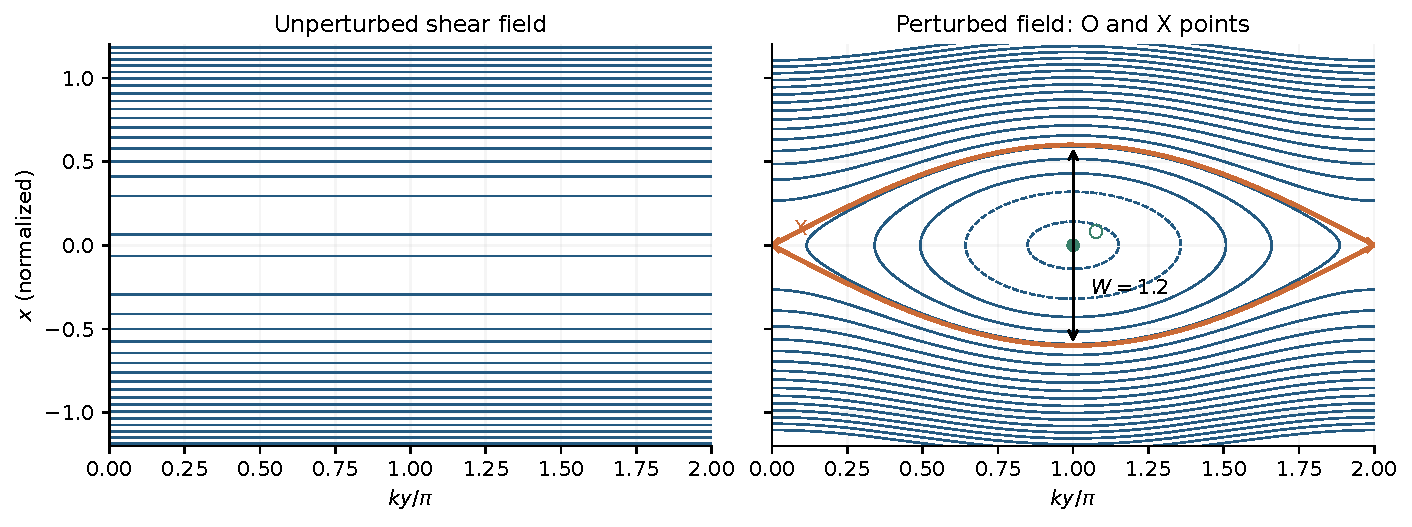
\includegraphics[width=\textwidth]{figures/tm_island.pdf}
\caption{由解析磁通函数直接绘制的磁岛。图采用无量纲$\psi=x^2/2+0.09\cos y$，所以全宽$W=4\sqrt{0.09}=1.2$。平面等值线、X/O点与分离线来自同一函数；这是教学解析图，不是实验照片或数值重联模拟。}
\label{tm:fig:island}
\end{figure}

\section{从MHD到磁通方程：不跳过符号}
从不可压、均匀密度、无黏性、标量电阻率的电阻MHD出发：
\begin{align}
 \rho(\partial_t\vct u+\vct u\cdot\nabla\vct u)&=-\nabla p+\J\times\B,\label{tm:momMHD}\\
 \E+\vct u\times\B&=\eta\J,\label{tm:ohmMHD}\\
 \partial_t\B&=-\nabla\times\E,\quad
 \mu_0\J=\nabla\times\B,\quad\nabla\cdot\B=0.
\end{align}
其中$\rho$为常数，$p$在不可压模型中负责维持$\nabla\cdot\vct u=0$；本章并未自洽计算温度。先这样简化，是为了单独看清电阻、惯性与磁剪切的作用，绝不是断言实验中的热流、黏性和双流体项总可忽略。

取矢势$A_z=-\psi$，则$\B=\nabla\times(-\psi\hat{\vct z})+B_g\hat{\vct z}$恰好符合式\eqref{tm:fluxstream}。由$\E=-\partial_t\vct A-\nabla\Phi_{\rm el}$，在$\partial_z\Phi_{\rm el}=0$规范下，$E_z=\partial_t\psi$。再逐项计算
\begin{equation}
 (\vct u\times\B)_z=u_xB_y-u_yB_x
 =-\phi_y\psi_x+\phi_x\psi_y=[\phi,\psi].
\end{equation}
将它与式\eqref{tm:current}代入欧姆律$z$分量，得
\begin{equation}
 \boxed{\partial_t\psi+[\phi,\psi]=D_\eta\nabla_\perp^2\psi.}
 \label{tm:induction}
\end{equation}
无电阻时右端为零，说明$\psi$被流场平流：$D\psi/Dt=0$。有电阻时，磁通可以相对于该流场改变。

可以给$\psi$加上只依赖时间的常数，磁场不变而$E_z$参考值改变；固定边界电压后该自由度也被固定。\textbf{二维重联的规范稳健量是X点与参考O点的磁通差。}移动的X/O点处$\nabla\psi=0$，所以
\begin{equation}
 \frac{\dd}{\dd t}(\psi_X-\psi_O)=E_z(X)-E_z(O).
 \label{tm:fluxrate}
\end{equation}
只有在参考电场可忽略或已明确扣除时，才可直接把$E_z(X)$叫作重联率。线性模的增长率$\gamma$则满足$\partial_t\widetilde\psi=\gamma\widetilde\psi$；它的单位是逆时间，不是电场单位。

\section{从动量方程到涡量方程：压力怎样被消去}
取式\eqref{tm:momMHD}的旋度。任意光滑标量满足$\nabla\times\nabla p=0$，因而压力梯度消失，但压力的力平衡作用没有被物理删除。二维不可压流的涡量沿$z$，没有涡量拉伸项，故惯性部分为
\begin{equation}
 \left[\nabla\times(\partial_t\vct u+\vct u\cdot\nabla\vct u)\right]_z
 =\partial_t\omega_z+\vct u\cdot\nabla\omega_z.
\end{equation}
这一等式也可用恒等式$\vct u\cdot\nabla\vct u=\nabla(u^2/2)-\vct u\times(\nabla\times\vct u)$逐项验证。

对磁力，在常数导场及仅有$J_z$的二维模型中，
\begin{equation}
 \J\times\B=J_z\hat{\vct z}\times(\hat{\vct z}\times\nabla\psi)
 =-J_z\nabla\psi.
\end{equation}
其旋度的$z$分量为
\begin{align}
 [\nabla\times(-J_z\nabla\psi)]_z
 &=-\partial_x(J_z\psi_y)+\partial_y(J_z\psi_x)\\
 &=-(J_{z,x}\psi_y+J_z\psi_{xy})+(J_{z,y}\psi_x+J_z\psi_{yx})\\
 &=\psi_xJ_{z,y}-\psi_yJ_{z,x}=[\psi,J_z].
\end{align}
两个含混合二阶导数的项恰好抵消。因此
\begin{equation}
 \boxed{\partial_t\nabla_\perp^2\phi+[\phi,\nabla_\perp^2\phi]
 =\frac{1}{\mu_0\rho}[\psi,\nabla_\perp^2\psi].}
 \label{tm:vortEq}
\end{equation}
式\eqref{tm:induction}和\eqref{tm:vortEq}构成下面使用的两场体系。二维不可压、常数导场情形下，它们直接来自上述MHD；在强导场、各向异性排序的三维问题中也会出现相关的约化MHD形式，但不能反过来把这两条二维式当成完整三维方程。\citep{TMLoureiro2007}

\section{选一个真正满足力平衡的电流片}
令
\begin{equation}
 B_{0y}(x)=B_0\tanh(x/a),\quad
 \psi_0(x)=B_0a\ln\cosh(x/a),\quad \phi_0=0.
 \label{tm:Harris}
\end{equation}
这里$B_0$是远离片中心的重联场，不是总导场。因为$\dd(\ln\cosh s)/\dd s=\tanh s$，第二式求导立即返回第一式。电流为
\begin{equation}
 J_{0z}(x)=\frac{B_0}{\mu_0a}\operatorname{sech}^2(x/a).
\end{equation}
再看$x$方向动量平衡：$0=-p_0'-J_{0z}B_{0y}$。用$J_{0z}=B_{0y}'/\mu_0$得
\begin{equation}
 \frac{\dd}{\dd x}\left(p_0+\frac{B_{0y}^2}{2\mu_0}\right)=0.
\end{equation}
因此
\begin{equation}
 p_0(x)=p_\infty+\frac{B_0^2}{2\mu_0}\operatorname{sech}^2(x/a).
\end{equation}
片中心磁压减少的部分被热压补上。常数导场只给总压增加常数，不改变这一平衡。

\paragraph{一个经常被省略的限制。}
在$D_\eta\ne0$且$\phi_0=0$时，$\partial_t\psi_0=D_\eta\psi_0''$，所以这不是永久静止的\emph{电阻}平衡。我们采用“冻结的背景近似”：平衡扩散时间$\tau_R=a^2/D_\eta$远长于模增长时间$\gamma^{-1}$。也可以明确加外源维持平衡，但那是另一种问题设定。后面必须检验$\gamma\tau_R\gg1$，而不能默默把平衡永远固定。

\section{归一化的每一个因子}
定义$V_A=B_0/\sqrt{\mu_0\rho}$、$\tau_A=a/V_A$，并令
\begin{equation}
 X=x/a,\quad Y=y/a,\quad \hat t=t/\tau_A,\quad
 \hat\psi=\psi/(B_0a),\quad \hat\phi=\phi/(V_Aa).
\end{equation}
磁通方程的时间项、平流项都具有量级$B_0V_A$，扩散项量级为$D_\eta B_0/a$。除以前者，得到系数
\begin{equation}
 \frac{D_\eta B_0/a}{B_0V_A}=\frac{D_\eta}{aV_A}=S_a^{-1},
 \qquad S_a\equiv\frac{aV_A}{D_\eta}=\frac{\tau_R}{\tau_A}.
\end{equation}
涡量方程两侧共同量级$V_A^2/a^2$，因为$B_0^2/(\mu_0\rho)=V_A^2$。故无量纲方程为
\begin{align}
 \partial_{\hat t}\hat\psi+[\hat\phi,\hat\psi]&=S_a^{-1}\hat\nabla_\perp^2\hat\psi,\\
 \partial_{\hat t}\hat\nabla_\perp^2\hat\phi+[\hat\phi,\hat\nabla_\perp^2\hat\phi]
 &=[\hat\psi,\hat\nabla_\perp^2\hat\psi].
\end{align}
这一步的实际作用是减少独立参数。改变$a,B_0,\rho,D_\eta$，只要$S_a$及边界、归一化波数相同，所选简化模型具有相同的无量纲线性问题；但真实等离子体的$d_i/a$、$\rho_i/a$与碰撞率可能同时改变，所以不能只看$S_a$就断言实验相似。

\chapter{线性化、共振面与外区驱动力}\label{tm:linear}
\section{什么是线性模，为什么用复指数}
设平衡量只依赖$x$，扰动沿$y$周期变化。用一个小参数$\epsilon_p$记录振幅阶数：
\begin{align}
 \psi(x,y,t)&=\psi_0(x)+\epsilon_p\operatorname{Re}\{\Psi(x)e^{iky+\gamma t}\},\\
 \phi(x,y,t)&=\epsilon_p\operatorname{Re}\{\Phi_c(x)e^{iky+\gamma t}\}.
 \label{tm:ansatz}
\end{align}
$\epsilon_p$与内层尺度$\delta/a$不是同一小参数。线性化只保留$O(\epsilon_p)$，删去两个扰动相乘的$O(\epsilon_p^2)$项。复数只是方便的记号，因为对一个模而言$\partial_y\to ik$、$\partial_t\to\gamma$；真实场总取实部。一般$\gamma$可为复数，实部代表增长，虚部代表相位传播。先研究静态对称平衡中的纯增长支$\gamma>0$，并不否认实验模会旋转。

定义
\begin{equation}
 F(x)\equiv\psi_0'(x)=B_{0y}(x),\qquad
 \mathcal L_k\equiv\frac{\dd^2}{\dd x^2}-k^2.
\end{equation}
本章撇号始终表示对有量纲$x$求导，故$F'$单位$\mathrm{T/m}$，$\Psi'$单位T。下一章若改用$X=x/a$会重新标明。

\section{磁通方程的线性化：把四项展开}
泊松括号展开为
\begin{equation}
 [\phi,\psi]=[0,\psi_0]+[\phi_1,\psi_0]+[0,\psi_1]+[\phi_1,\psi_1].
\end{equation}
第一、三项为零，最后一项为二阶小量。由于$\partial_y\psi_0=0$，中间保留项为
\begin{equation}
 [\phi_1,\psi_0]=(\partial_x\phi_1)\underbrace{\partial_y\psi_0}_{0}
 -(\partial_y\phi_1)\partial_x\psi_0=-ikF\Phi_c e^{iky+\gamma t}.
\end{equation}
背景扩散属于零阶平衡方程，扣除背景后得到
\begin{equation}
 \boxed{\gamma\Psi=ikF\Phi_c+D_\eta\mathcal L_k\Psi.}
 \label{tm:linind}
\end{equation}
这里保留了$k^2\Psi$。在薄内层中稍后可以通过$k\delta\ll1$删除它；\textbf{在外区不能提前删掉}，否则会丢失远处衰减与波长稳定阈值。

\section{涡量方程的线性化：电流梯度从哪里来}
因为平衡流为零，左侧非线性平流$[\phi,\nabla^2\phi]$完全是二阶。右侧有两项一阶贡献：
\begin{align}
 [\psi,\nabla^2\psi]_1
 &=[\psi_0,\nabla^2\psi_1]+[\psi_1,\nabla^2\psi_0],\\
 [\psi_0,\nabla^2\psi_1]&=F\,ik\mathcal L_k\Psi\,e^{iky+\gamma t},\\
 [\psi_1,\nabla^2\psi_0]&=-ik\Psi\,\frac{\dd}{\dd x}(\psi_0'')e^{iky+\gamma t}
 =-ikF''\Psi e^{iky+\gamma t}.
\end{align}
于是
\begin{equation}
 \boxed{\gamma\mathcal L_k\Phi_c
 =\frac{ik}{\mu_0\rho}\left(F\mathcal L_k\Psi-F''\Psi\right).}
 \label{tm:linvort}
\end{equation}
$F''=\mu_0J_{0z}'$正是平衡电流梯度信息。若只保留$F\Psi''$而把$F''\Psi$到处删除，就不能正确计算外区驱动力。近片中心的内层可因局部线性磁剪切忽略$F''$；这个局部事实不能推广到整个电流片。

对于纯增长的对称撕裂支，可令$\Psi$为实函数并写$\Phi_c=-i\Phi$，其中$\Phi$也为实函数。这对应磁通扰动为$\Psi\cos ky$，流函数为$\Phi\sin ky$。代入后得到实方程
\begin{align}
 \gamma\Psi&=kF\Phi+D_\eta\mathcal L_k\Psi,\label{tm:realind}\\
 \gamma\mathcal L_k\Phi&=-\frac{k}{\mu_0\rho}
 \left(F\mathcal L_k\Psi-F''\Psi\right).
 \label{tm:realvort}
\end{align}
第二式的负号来自将两边共同的$i$约去，而不是任意选择。对于奇函数$F$，撕裂支的$\Psi(x)$为偶函数、$\Phi(x)$为奇函数；两侧流动围绕磁岛有相应奇偶性。

\section{共振面为什么是内外区分界}
沿平衡磁场对一个扰动求导：
\begin{equation}
 \B_0\cdot\nabla(\widetilde f e^{iky+ik_zz})
 =i(kF+k_zB_g)\widetilde f e^{iky+ik_zz}.
\end{equation}
磁张力沿场传递，因而$kF+k_zB_g=0$处的沿场恢复作用有特殊性；此处称共振面。在本讲义的二维$k_z=0$问题中，共振面就是$F=0$，对Harris片为$x=0$。有导场并不使这一二维共振面消失；若允许斜模$k_z\ne0$，共振面位置就会改变。

设外区电阻很小，先从式\eqref{tm:realind}得到
\begin{equation}
 \Phi\simeq\frac{\gamma\Psi}{kF}.
 \label{tm:idealflow}
\end{equation}
如果$\Psi(0)\ne0$且$F\simeq B'_0x$，这个理想解在$x\to0$时像$1/x$发散。这并不是实际流速无限大，而是告诉我们：\textbf{删掉电阻的近似在这里失效}。小电阻乘上很大的磁通二阶导数，仍可以与时间项同阶。薄层内还必须保留惯性，否则无法决定增长时标。这就是奇异摄动，而不是在全域给理想解简单加一个很小修正。

\paragraph{类比，但只作理解。}
在一根几乎没有电阻的导线上，绝大部分电压降可以集中在一个很短的电阻段；“段很短”不等于“段不重要”。撕裂内层同样可以很薄，却决定拓扑改变与增长率。外区仍不可省略，因为它决定有多少自由能和何种边界响应能供给内层。

\section{外区近似的时间排序}
令$\tau_A=a/V_A$、$\tau_R=a^2/D_\eta$，假设
\begin{equation}
 \tau_A\ll\gamma^{-1}\ll\tau_R,
 \qquad\text{即}\qquad S_a^{-1}\ll\hat\gamma\ll1,
 \quad \hat\gamma\equiv\gamma\tau_A.
 \label{tm:outerordering}
\end{equation}
右边不等式使外区在模明显增长之前已能近似完成Alfv\'en力平衡；左边不等式使背景尚未显著电阻扩散。若沿片波数很小，还须检查模相对于沿片Alfv\'en时间的慢排序$\gamma\ll kV_A$，不能只检查$\hat\gamma\ll1$。

在$|x|\sim a$，$\mathcal L_k\sim a^{-2}$（$ka=O(1)$）且由式\eqref{tm:idealflow}，$\Phi\sim\gamma\Psi/(kB_0)$。惯性与磁力之比估计为
\begin{equation}
 \frac{\gamma\Phi/a^2}{kB_0\Psi/(\mu_0\rho a^2)}
 \sim\frac{\gamma^2\mu_0\rho}{k^2B_0^2}
 =\left(\frac{\gamma}{kV_A}\right)^2\ll1.
\end{equation}
因此外区涡量式右端应近似为零：
\begin{equation}
 F(\Psi''-k^2\Psi)-F''\Psi=0.
\end{equation}
在$F\ne0$处除以$F$，得到\emph{外区撕裂方程}
\begin{equation}
 \boxed{\Psi''-\left(k^2+\frac{F''}{F}\right)\Psi=0.}
 \label{tm:outerode}
\end{equation}
它是二阶常微分方程，不含$\gamma$，所以\textbf{外区本身决定不了增长率}。它计算的是近似静态磁力平衡对薄层磁通扰动的响应。\citep{TMFitzMatching}

\section{\texorpdfstring{$\Delta'$}{Delta prime}的定义：比较的是两侧斜率}
分别在$x>0$与$x<0$解式\eqref{tm:outerode}，要求远离电流片时扰动衰减（或满足实际壁面条件）。由于线性问题的总振幅任意，可以把两侧解都归一成$\Psi(0)=\Psi_s$。两侧函数值相同，但外区延拓到零点后的导数一般不同。定义
\begin{equation}
 \boxed{\Delta'\equiv
 \frac{\Psi'(0^+)-\Psi'(0^-)}{\Psi_s}.}
 \label{tm:deltaprime}
\end{equation}
这里$0^\pm$是\emph{外区解向薄层中心的渐近延拓}，并不说真实磁场在中心有物理无限薄的不连续面。真实内区将这处斜率差平滑连接。$\Delta'$单位为$\mathrm{m^{-1}}$，$\Delta'a$才无量纲。

在重叠区$\delta\ll|x|\ll a$，偶对称解具有
\begin{equation}
 \Psi_{\rm out}(x)=\Psi_s\left(1+\frac{\Delta'}{2}|x|+\cdots\right).
 \label{tm:outermatch}
\end{equation}
内区解的远场也必须给出相同常数项与线性斜率。这一“相同区域中表示同一个函数”的要求叫渐近匹配。不能把两条图线在任选一点简单接起来当成匹配。

还可用积分读出$\Delta'$：跨过内层，
\begin{equation}
 \int_{-\ell}^{\ell}\Psi''\,\dd x
 =\Psi'(\ell)-\Psi'(-\ell)\longrightarrow\Delta'\Psi_s,
 \quad \delta\ll\ell\ll a.
 \label{tm:currentjump}
\end{equation}
由$\mu_0\widetilde J_z=\Psi''-k^2\Psi$，它约束薄层中扰动电流的积分。$k^2$项的积分相对薄层二阶导数项为小量，删除它须依赖薄层排序。

在这里研究的经典静态、无压强曲率驱动、无流剪切电阻问题中，$\Delta'>0$给出不稳定撕裂支；$\Delta'<0$没有该自发增长支。这个结论不能无条件推广到新经典撕裂模、受迫重联、漂移或流剪切驱动问题。负$\Delta'$的系统仍可被外部共振磁扰动强迫产生磁岛。

\begin{figure}[htbp]
\centering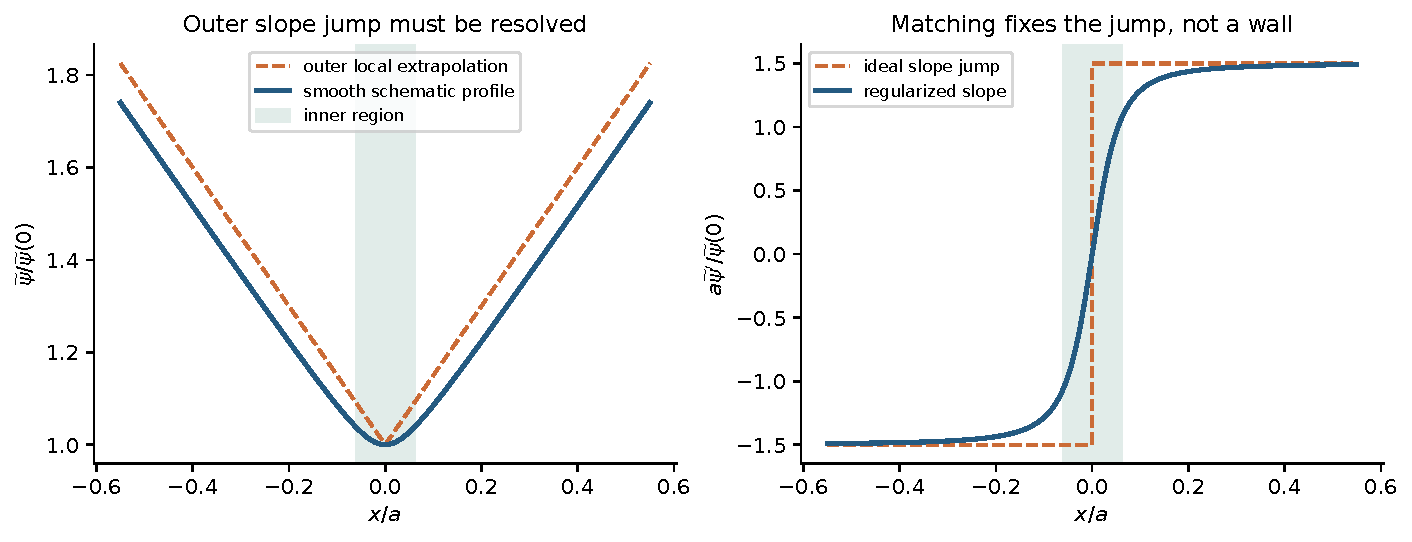
\includegraphics[width=\textwidth]{figures/tm_matching.pdf}
\caption{内外区匹配的几何示意，选取$\Delta'a=3$与$\delta/a=0.06$。红色曲线是为了展示“相同远场斜率、不同内层平滑”而构造的正则化函数，不是已求解的FKR内区本征函数，不能从图中读出精确层宽或增长率。}
\label{tm:fig:matching}
\end{figure}

\section{Harris片的外区解：从候选函数逐项验算}
对$F=B_0\tanh(x/a)$，令$X=x/a$、$K=ka$。因为
\begin{align}
 F'&=\frac{B_0}{a}\operatorname{sech}^2X,\\
 F''&=-\frac{2B_0}{a^2}\operatorname{sech}^2X\tanh X,
\end{align}
所以$F''/F=-2\operatorname{sech}^2X/a^2$。在$X=0$，分子与分母都趋零，但这个比值有有限极限；不要把形式上的$0/0$误认为外区系数必有无穷大。

式\eqref{tm:outerode}变为
\begin{equation}
 \frac{\dd^2\Psi}{\dd X^2}-\left(K^2-2\operatorname{sech}^2X\right)\Psi=0.
 \label{tm:harrisode}
\end{equation}
在$X>0$试取会在无穷远衰减的函数
\begin{equation}
 f_+(X)=e^{-KX}(K+\tanh X).
\end{equation}
为避免一行带过，令$T=\tanh X$、$Q=\operatorname{sech}^2X=1-T^2$，则$T'=Q$、$Q'=-2TQ$。两次求导：
\begin{align}
 f_+'&=e^{-KX}\{Q-K(K+T)\},\\
 f_+''&=e^{-KX}\{-2TQ-2KQ+K^2(K+T)\}\\
 &=e^{-KX}(K+T)(K^2-2Q)=(K^2-2Q)f_+.
\end{align}
这正是式\eqref{tm:harrisode}，所以候选函数是精确外区解。负侧由偶对称给出$f_-(X)=f_+(-X)$。统一归一化后，
\begin{equation}
 \frac{\Psi(X)}{\Psi_s}=e^{-K|X|}\left(1+\frac{\tanh|X|}{K}\right).
 \label{tm:harrissolution}
\end{equation}
注意它不是$e^{-K|X|}$一项；后面的$\tanh$因子携带电流片内部的响应。

在$X=0^+$，$f_+(0)=K$、$f_+'(0)=1-K^2$。将无量纲导数换回$\dd/\dd x=a^{-1}\dd/\dd X$，
\begin{align}
 \frac{\Psi'(0^+)}{\Psi_s}&=\frac{1}{a}\left(\frac1K-K\right),\\
 \frac{\Psi'(0^-)}{\Psi_s}&=-\frac{1}{a}\left(\frac1K-K\right),\\
 \boxed{\Delta'a=2\left(\frac1K-K\right).}
 \label{tm:harrisdelta}
\end{align}
因此无限域Harris片的经典撕裂不稳定波数满足$0<ka<1$，等价于$\lambda>2\pi a$。在有限周期盒长$L_y$中，允许波数为$k_m=2\pi m/L_y$；是否有不稳定模还要看盒内是否容得下这些波长。

\paragraph{算完三个波长与一个盒长。}
取$a=0.10\,\mathrm m$。$ka=0.5$时$k=5\,\mathrm{m^{-1}}$、$\lambda=1.257\,\mathrm m$、$\Delta'a=3$、$\Delta'=30\,\mathrm{m^{-1}}$。$ka=1$时$\lambda=0.628\,\mathrm m$、$\Delta'=0$。$ka=2$时$\lambda=0.314\,\mathrm m$、$\Delta'a=-3$，没有此经典增长支。

若取$L_y=2.0\,\mathrm m$，则$K_m=0.31416m$：$m=1,2,3$的$K$分别为$0.314,0.628,0.942$，都满足$K<1$；$m=4$的$K=1.257$不满足。这里的$m$是沿片周期盒模数，不是后文托卡马克的极向模数。它们同用字母只因都表示整数傅里叶谐波。

\begin{figure}[htbp]
\centering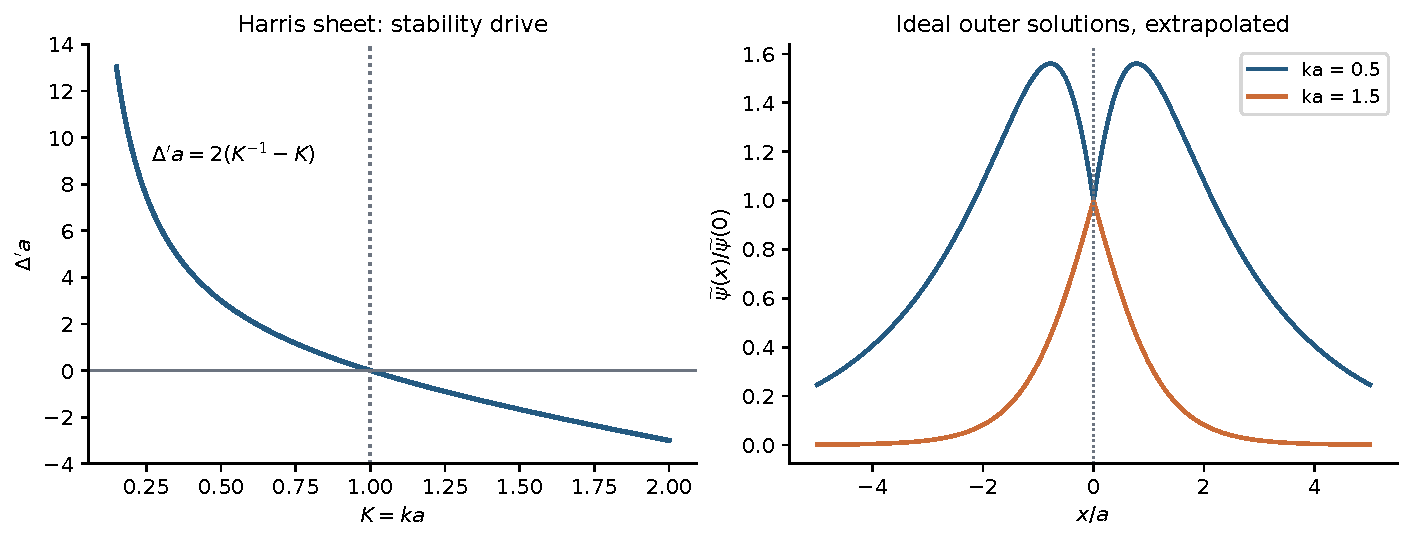
\includegraphics[width=\textwidth]{figures/tm_harris_delta.pdf}
\caption{Harris平衡的解析外区解和$\Delta'a=2(1/K-K)$。中心处折角是忽略内层后得到的两侧渐近解，不是真实无限薄电流奇点；内层将其平滑连接。右图的稳定性判据限定于本章经典无流、无限域问题。}
\label{tm:fig:harris}
\end{figure}

\section{正\texorpdfstring{$\Delta'$}{Delta prime}的物理意义与边界依赖}
当$K<1$时，式\eqref{tm:harrissolution}在中心右侧先向上弯出正斜率，左侧斜率相反。外区希望薄层提供与这种斜率差相容的扰动电流；电阻允许该电流结构随拓扑变化建立，惯性决定流动响应有多快。用“外区提供驱动、内区决定通道和时标”记住分工，比把$\Delta'$只当一个背诵的稳定性符号更有用。

$\Delta'$不是局地点只测$B'_0$就能知道的量。它来自从两侧边界积分到共振面，所以改变导体壁位置、电流剖面、压力曲率或其他共振面，可能改变它甚至改变符号。Harris解析式是一个明确平衡与无限域边界下的结果；不能只因实际磁场在中心近似线性，就对任意装置使用$2(K^{-1}-K)$。

\paragraph{本章学到哪一步。}
现在我们已经知道哪个波长具有经典撕裂驱动，也得到内区必须满足的电流积分。我们\emph{还不知道}$\gamma$与$\delta$。这不是推导缺了一项数值系数，而是外区方程按构造就删掉了决定时标的惯性与电阻；下一章必须把它们取回来。

\chapter{薄内层怎样选出增长率：从标度到匹配常数}\label{tm:matching}
\section{先列近似，再删项}
本章取$\gamma>0$、$\Delta'>0$的经典撕裂支。近共振面，$F=B_{0y}\simeq B'_0x$，Harris片有$B'_0=B_0/a$。假设内层$|x|\sim\delta\ll a$，同时$k\delta\ll1$。在适当薄层排序下，$k^2\Psi$小于横向二阶导数，$F''\Psi$小于$F\Psi''$；但$D_\eta\Psi''$与惯性$\gamma\Phi''$不能再删。式\eqref{tm:realind}--\eqref{tm:realvort}约化为
\begin{align}
 \gamma\Psi&=kB'_0x\Phi+D_\eta\Psi'',\label{tm:inner1}\\
 \gamma\Phi''&=-\frac{kB'_0}{\mu_0\rho}x\Psi''.
 \label{tm:inner2}
\end{align}
必须同时求解两条式子。只用“扩散时间等于增长时间”会漏掉磁张力和流体惯性，因此得不到FKR的$3/5$指数。

下面把$X=x/a$、$K=ka$、$\epsilon=\delta/a$、$\hat\gamma=\gamma a/V_A$、$\Delta=\Delta'a$作为简记。磁通和流函数分别按$B_0a$、$V_Aa$归一化，两条内层方程成为
\begin{align}
 \hat\gamma\Psi&=KX\Phi+S_a^{-1}\Psi_{XX},\label{tm:innernorm1}\\
 \hat\gamma\Phi_{XX}&=-KX\Psi_{XX}.
 \label{tm:innernorm2}
\end{align}
这里为便于阅读，$\Psi,\Phi$暂省去归一化帽号，但导数明确写成$XX$。有量纲公式会重新标出。

\section{常磁通近似并不是磁场不变}
设内层跨越时磁通扰动仅有小变化：$\Psi(X)=\Psi_s+\psi_c(X)$，$|\psi_c|\ll|\Psi_s|$。由外区匹配，导数跳跃为$\Delta\Psi_s$，而跳跃发生在尺度$\epsilon$内，因此
\begin{equation}
 \Psi_{XX}\sim\frac{\Delta\Psi_s}{\epsilon},\qquad
 \psi_c\sim\Psi_{XX}\epsilon^2\sim\Delta\epsilon\Psi_s.
 \label{tm:constpsiscaling}
\end{equation}
所以常磁通（constant-$\psi$）条件是
\begin{equation}
 \boxed{\Delta'\delta=\Delta\epsilon\ll1.}
 \label{tm:constpsicond}
\end{equation}
它表示\emph{磁通扰动振幅}在层内近似常数。它并不表示$\Psi'=0$、电流为零或没有重联。微小变化除以微小层宽后，二阶导数仍可很大。

一个数值类比：取归一化磁通变化$\psi_c/\Psi_s=0.01$、层宽$\epsilon=0.005$，则$\Psi_{XX}/\Psi_s\sim0.01/(0.005)^2=400$。函数值只变1\%，二阶导数却达到400；在内层保留电阻项毫不矛盾。

\section{FKR标度：三个平衡，逐步消去未知量}
由涡量式\eqref{tm:innernorm2}，取$X\sim\epsilon$、$\Phi_{XX}\sim\Phi/\epsilon^2$并使用式\eqref{tm:constpsiscaling}，得到
\begin{equation}
 \hat\gamma\frac{\Phi}{\epsilon^2}
 \sim K\epsilon\frac{\Delta\Psi_s}{\epsilon}
 =K\Delta\Psi_s.
\end{equation}
因此
\begin{equation}
 \Phi\sim\frac{K\Delta\epsilon^2}{\hat\gamma}\Psi_s.
 \label{tm:phiscale}
\end{equation}
磁通式中的时间项、电阻项与平流项共同参与主阶平衡。时间与电阻比较：
\begin{equation}
 \hat\gamma\Psi_s\sim S_a^{-1}\frac{\Delta\Psi_s}{\epsilon}
 \quad\Rightarrow\quad
 \hat\gamma\sim S_a^{-1}\frac{\Delta}{\epsilon}.
 \label{tm:resbalance}
\end{equation}
时间与平流比较，并代入式\eqref{tm:phiscale}：
\begin{equation}
 \hat\gamma\Psi_s\sim K\epsilon\Phi
 \sim\frac{K^2\Delta\epsilon^3}{\hat\gamma}\Psi_s
 \quad\Rightarrow\quad
 \hat\gamma^2\sim K^2\Delta\epsilon^3.
 \label{tm:advbalance}
\end{equation}
把式\eqref{tm:resbalance}平方，代入式\eqref{tm:advbalance}：
\begin{align}
 S_a^{-2}\frac{\Delta^2}{\epsilon^2}&\sim K^2\Delta\epsilon^3,\\
 \epsilon^5&\sim S_a^{-2}\Delta K^{-2},\\
 \boxed{\epsilon\sim S_a^{-2/5}\Delta^{1/5}K^{-2/5}.}\label{tm:FKRdelta}
\end{align}
再代回$\hat\gamma\sim S_a^{-1}\Delta/\epsilon$，逐个合并幂指数：
\begin{equation}
 \boxed{\hat\gamma\sim
 S_a^{-1+2/5}\Delta^{1-1/5}K^{2/5}
 =S_a^{-3/5}\Delta^{4/5}K^{2/5}.}
 \label{tm:FKRgamma}
\end{equation}
这就是经典常磁通电阻撕裂标度。$\gamma\propto D_\eta^{3/5}$说明电阻趋零时，在\emph{固定厚度、固定波数、固定外区驱动}条件下增长率趋零。后面薄片的厚度本身随$S$变化时，不能沿用这个“固定几何”的解释。

\paragraph{回查刚才删掉的$k^2$项。}
在常磁通层内，$k^2\Psi/\Psi''\sim K^2\epsilon/\Delta$。通常远离$\Delta=0$且层很薄时满足小量；但靠近边际$K\to1$，$\Delta$很小，不能只凭$k\delta\ll1$就保证所有删项。FKR公式在严格边际附近与更高阶效应的次序，应重新核对，而非任意精确外推到$\Delta=0$附近。

\section{再前进一步：常磁通匹配系数不是随意拟合}
上节的$\sim$没有决定$O(1)$系数。本节给出其来源；若首次阅读不熟悉特殊函数，可以先掌握式\eqref{tm:FKRexact}，随后沿下面的步骤复算。这里的数学稍深，但没有增加新的物理假设。

回到有量纲式\eqref{tm:inner1}，在时间项中取$\Psi\simeq\Psi_s$，但\emph{仍保留}$\Psi''$。定义
\begin{equation}
 \delta_*\equiv\left[\frac{\mu_0\rho D_\eta\gamma}{k^2(B'_0)^2}\right]^{1/4},
 \quad \xi=\frac{x}{\delta_*},\quad
 \Phi(x)=\frac{\gamma\Psi_s}{kB'_0\delta_*}\,f(\xi).
 \label{tm:deltastar}
\end{equation}
$\delta_*$是一种明确的内层特征尺度，不是电流半高全宽；不同论文对“层宽”的定义会给不同数值系数。由磁通式直接得到
\begin{equation}
 \Psi''=\frac{\gamma\Psi_s}{D_\eta}[1-\xi f(\xi)].
 \label{tm:psisecond}
\end{equation}
再将它与$\Phi''=\gamma\Psi_s f''/(kB'_0\delta_*^3)$代入涡量式，除去公共系数：
\begin{equation}
 f''=-\frac{k^2(B'_0)^2\delta_*^4}{\mu_0\rho D_\eta\gamma}\,\xi(1-\xi f)
 =-\xi(1-\xi f).
\end{equation}
所以需要求解的\emph{无参数}内层形状方程是
\begin{equation}
 \boxed{f''-\xi^2f=-\xi,\qquad f(-\xi)=-f(\xi),\quad
 f(\xi)\sim\xi^{-1}\ (|\xi|\to\infty).}
 \label{tm:shapeODE}
\end{equation}
远场条件来自理想关系$\Phi=\gamma\Psi_s/(kB'_0x)$；不是任意设定的边界条件。

将式\eqref{tm:psisecond}跨内层积分，再用式\eqref{tm:currentjump}匹配，
\begin{align}
 \Delta'\Psi_s&=\frac{\gamma\Psi_s\delta_*}{D_\eta}
 \int_{-\infty}^{\infty}[1-\xi f(\xi)]\,\dd\xi,\\
 \Delta'&=I\frac{\gamma\delta_*}{D_\eta},\qquad
 I\equiv\int_{-\infty}^{\infty}[1-\xi f(\xi)]\,\dd\xi.
 \label{tm:matchI}
\end{align}
$\Psi_s$完全约去，所以线性增长率不依赖任意选择的小种子振幅。种子影响需要等待多久才达到非线性幅度，却不改变这里的本征增长率。

\subsection{通过正弦变换求\texorpdfstring{$I$}{I}}
令$\mathcal F(p)=\int_0^\infty f(\xi)\sin(p\xi)\,\dd\xi$，其中$p>0$是\emph{内层坐标}$\xi$的变换变量，和沿片波数$k$不同。积分可先乘$e^{-\varepsilon\xi}$，计算后令$\varepsilon\to0^+$，以正确处理$f\sim1/\xi$的远场。

两次分部积分给$\int f''\sin(p\xi)\dd\xi=-p^2\mathcal F$，而对$p$两次求导给$\int\xi^2f\sin(p\xi)\dd\xi=-\mathcal F''$。式\eqref{tm:shapeODE}右端$-\xi$的带阻尼变换在固定$p>0$后取极限为零，故
\begin{equation}
 \mathcal F''-p^2\mathcal F=0\quad(p>0).
\end{equation}
远场$f\sim1/\xi$决定$\mathcal F(0^+)=\pi/2$。这个值可以从
$\int_0^\infty e^{-\varepsilon\xi}\sin(p\xi)\dd\xi/\xi
=\arctan(p/\varepsilon)$看出；在$\varepsilon\to0^+$后得到$\pi/2$。还要求$\mathcal F(p)$在$p\to\infty$衰减。

令$z=p^2/2$、$\mathcal F=\sqrt p\,H(z)$。为避免跳过链式法则，这里把两次求导写开（$H'$对$z$求导）：
\begin{align*}
 \mathcal F'&=\frac{H}{2\sqrt p}+p^{3/2}H',\\
 \mathcal F''&=-\frac{H}{4p^{3/2}}+2p^{1/2}H'+p^{5/2}H''.
\end{align*}
将$\mathcal F''-p^2\mathcal F=0$除以$p^{5/2}$得
$H''+(2/p^2)H'-(1+1/(4p^4))H=0$。再用$p^2=2z$并乘$z^2$，得到
\begin{equation}
 z^2H''+zH'-(z^2+1/16)H=0.
\end{equation}
这是阶数$1/4$的修正Bessel方程；其衰减解记为$K_{1/4}(z)$。它可以用积分定义：
\begin{equation*}
 K_\nu(z)=\int_0^\infty e^{-z\cosh t}\cosh(\nu t)\dd t.
\end{equation*}
它只是上述微分方程的函数解，并非另外一个物理模型。因此
\begin{equation}
 \mathcal F(p)=C\sqrt p\,K_{1/4}(p^2/2).
\end{equation}
在$p\to0^+$，由此函数的两个独立小参数幂解，
\begin{equation}
 \sqrt p\,K_{1/4}(p^2/2)
 =\frac{\Gamma(1/4)}{\sqrt2}
 +\frac{\Gamma(-1/4)}{2\sqrt2}\,p+O(p^4).
\end{equation}
$\Gamma$是Gamma函数，$\Gamma(s)=\int_0^\infty t^{s-1}e^{-t}\dd t$（先取$s>0$，其余用递推延拓）。分部积分给$\Gamma(s+1)=s\Gamma(s)$，故$\Gamma(-1/4)=-4\Gamma(3/4)$。归一化$\mathcal F(0^+)=\pi/2$后，
\begin{equation}
 \mathcal F'(0^+)=-\pi\frac{\Gamma(3/4)}{\Gamma(1/4)}.
\end{equation}
由于$1-\xi f$为偶函数，且其半轴余弦变换在$p>0$为$-\mathcal F'(p)$，令$p\to0^+$便得到
\begin{equation}
 \boxed{I=-2\mathcal F'(0^+)
 =2\pi\frac{\Gamma(3/4)}{\Gamma(1/4)}=2.12364827.}
\end{equation}
这里对常数1的变换也要使用同一阻尼极限；不能把两个分别不收敛的积分先随意拆开，再分别令$p=0$。

\subsection{解出含系数的增长率}
把式\eqref{tm:deltastar}代入式\eqref{tm:matchI}：
\begin{equation}
 \Delta'=I\gamma^{5/4}D_\eta^{-3/4}
 \left(\frac{kB'_0}{\sqrt{\mu_0\rho}}\right)^{-1/2}.
\end{equation}
两边乘相应系数再取$4/5$次方，得
\begin{equation}
 \gamma=I^{-4/5}D_\eta^{3/5}
 \left(\frac{kB'_0}{\sqrt{\mu_0\rho}}\right)^{2/5}(\Delta')^{4/5}.
\end{equation}
对于$B'_0=B_0/a$，无量纲形式为
\begin{align}
 \boxed{\gamma\tau_A=C_\gamma S_a^{-3/5}K^{2/5}\Delta^{4/5},\quad
 C_\gamma=I^{-4/5}=0.547436725,}\label{tm:FKRexact}\\
 \frac{\delta_*}{a}=C_\delta S_a^{-2/5}K^{-2/5}\Delta^{1/5},\quad
 C_\delta=I^{-1/5}=0.860168397.
 \label{tm:FKRwidthexact}
\end{align}
这些系数属于本章无黏性、常磁通、局部线性剪切与明确宽度定义；改变闭合或层宽定义时，不应坚持使用同一个数值系数。经典FKR关系的物理来源与现代匹配写法见原始文献及作者讲义。\citep{TMFKR1963,TMFitzMatching}

\section{大\texorpdfstring{$\Delta'$}{Delta prime}：为什么必须换一套估计}
如果算出$\Delta'\delta\gtrsim1$，磁通在层内不能再近似不变。此时应取
\begin{equation}
 \Psi_{XX}\sim\frac{\Psi}{\epsilon^2},
\end{equation}
而不是$\Delta\Psi/\epsilon$。仍用同一两条内层方程，涡量平衡给
\begin{equation}
 \hat\gamma\frac{\Phi}{\epsilon^2}\sim K\epsilon\frac{\Psi}{\epsilon^2}
 \quad\Rightarrow\quad \Phi\sim\frac{K\epsilon}{\hat\gamma}\Psi.
\end{equation}
磁通的时间和平流项平衡给
$\hat\gamma\Psi\sim K\epsilon\Phi$，所以$\hat\gamma^2\sim K^2\epsilon^2$，取增长支$\hat\gamma\sim K\epsilon$。时间与电阻平衡给$\hat\gamma\sim S_a^{-1}\epsilon^{-2}$。两者相等：
\begin{align}
 K\epsilon&\sim S_a^{-1}\epsilon^{-2},\\
 \boxed{\frac{\delta}{a}\sim S_a^{-1/3}K^{-1/3},\qquad
 \gamma\tau_A\sim S_a^{-1/3}K^{2/3}.}
 \label{tm:Coppi}
\end{align}
这通常称大$\Delta'$或Coppi型区间。增长率的主阶不再显式依赖$\Delta'$，并不意味着外区消失；外区仍负责确保驱动足够大、允许该匹配极限。这里没有给一般有限$\Delta'$色散关系的精确数值常数。图中的系数1只用于量级比较。\citep{TMLoureiro2007}

\section{两个区间在哪里相遇，为什么有最快波长}
对Harris片长波$K\ll1$，$\Delta\simeq2/K$。FKR增长率因此满足
\begin{equation}
 \hat\gamma_{\rm FKR}\sim S_a^{-3/5}K^{2/5}(K^{-1})^{4/5}
 \sim S_a^{-3/5}K^{-2/5}.
\end{equation}
在这一支上，减小$K$（加长波长）使增长变快；但大$\Delta'$支满足$\hat\gamma\sim S_a^{-1/3}K^{2/3}$，减小$K$反而变慢。最快模应在两种平衡的过渡附近，而不是$K\to0$。

用常磁通失效条件$\Delta\epsilon\sim1$，
\begin{equation}
 K^{-1}S_a^{-2/5}K^{-1/5}K^{-2/5}
 =S_a^{-2/5}K^{-8/5}\sim1,
\end{equation}
得到
\begin{equation}
 \boxed{K_*\sim S_a^{-1/4},\qquad
 \hat\gamma_*\sim S_a^{-1/2},\qquad \delta_*/a\sim S_a^{-1/4}.}
 \label{tm:fastest}
\end{equation}
这里用的是幂次关系，忽略的$O(1)$系数会移动峰值；不能把两个渐近式的交点称为已经精确求得的本征谱。若盒长不允许这个$K_*$，最快的\emph{实际允许模}还要在离散$k_m$中选择。

\begin{figure}[htbp]
\centering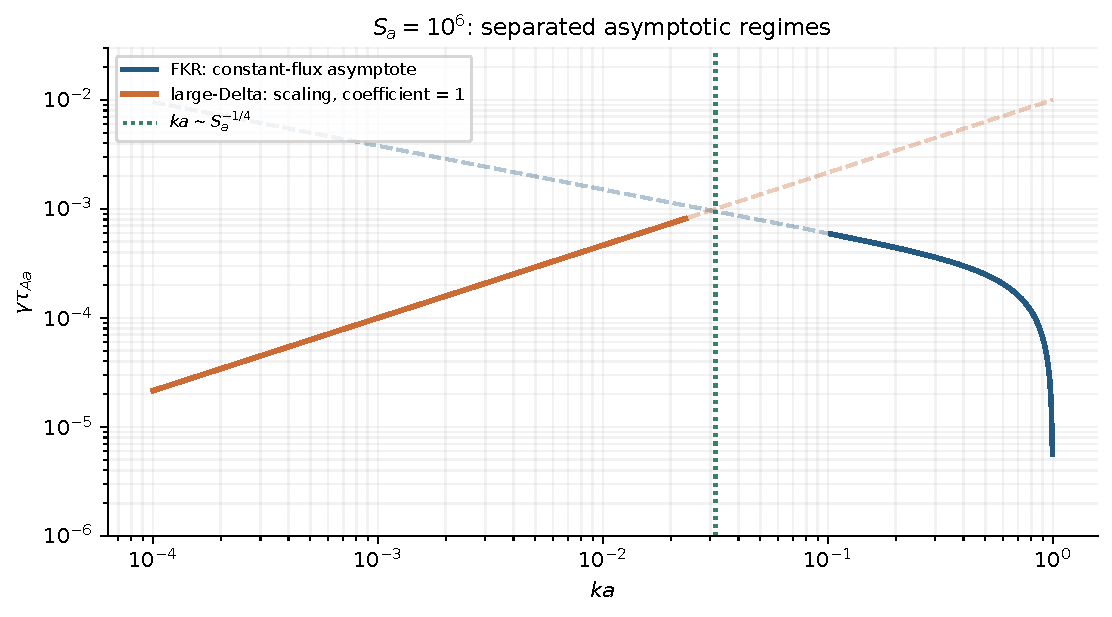
\includegraphics[width=\textwidth]{figures/tm_fkr_coppi.pdf}
\caption{$S_a=10^6$时两种渐近增长率。FKR支使用本章导出的$C_\gamma=0.5474367$；大$\Delta'$支取系数1以示量级。实线分别限制在图中所选的$\Delta'\delta<0.3$或$>3$区间，虚线是超出该条件的形式延拓；中间区域须另解完整本征问题，不能把曲线交点当精确最快模。}
\label{tm:fig:regimes}
\end{figure}

\section{完整数值算例一：得到答案后逐项检查}
本节是\textbf{自行指定系数的数学MHD教学算例}，不冒充某次实验。取
\begin{equation}
 a=0.10\,\mathrm m,\quad V_A=10^5\,\mathrm{m/s},\quad
 D_\eta=0.010\,\mathrm{m^2/s},\quad K=ka=0.50.
\end{equation}
则$\eta=\mu_0D_\eta=1.2566\times10^{-8}\,\Omega\,\mathrm m$，
\begin{align}
 S_a&=\frac{0.10\times10^5}{0.010}=10^6,\\
 \tau_A&=\frac{0.10}{10^5}=10^{-6}\,\mathrm s,\qquad
 \tau_R=\frac{(0.10)^2}{0.010}=1.0\,\mathrm s,\\
 k&=5.0\,\mathrm{m^{-1}},\quad\lambda=1.257\,\mathrm m,\quad
 \Delta=2(2-0.5)=3.
\end{align}
代入含系数FKR公式，
\begin{align}
 \gamma\tau_A&=0.5474367\,(10^6)^{-3/5}(0.5)^{2/5}3^{4/5}
 =2.50968\times10^{-4},\\
 \boxed{\gamma=250.97\,\mathrm{s^{-1}},\quad\gamma^{-1}=3.985\,\mathrm{ms}},\\
 \frac{\delta_*}{a}&=0.8601684\,(10^6)^{-2/5}(0.5)^{-2/5}3^{1/5}
 =0.00562885,\\
 \boxed{\delta_*=5.629\times10^{-4}\,\mathrm m=0.563\,\mathrm{mm}.}
\end{align}
现在检查，而不是把数字算完就结束：
\begin{align}
 \gamma\tau_A&=2.51\times10^{-4}\ll1,&\gamma\tau_R&=251\gg1,\\
 \delta_*/a&=0.00563\ll1,&k\delta_*&=0.00281\ll1,\\
 \Delta'\delta_*&=\Delta\delta_*/a=0.0169\ll1,&
 \gamma/(kV_A)&=5.02\times10^{-4}\ll1.
\end{align}
所用几何、时间、常磁通与沿片慢排序均较好满足。$k^2\Psi/\Psi''\sim K^2\epsilon/\Delta=4.69\times10^{-4}$，也很小。

无黏性还需要额外检验。如果加入运动黏度$\nu$，涡量式多出$\nu\nabla^4\phi$，内层黏性/惯性比为
\begin{equation}
 \frac{\nu\Phi/\delta_*^4}{\gamma\Phi/\delta_*^2}
 =\frac{\nu}{\gamma\delta_*^2}.
\end{equation}
本例$\gamma\delta_*^2=7.95\times10^{-5}\,\mathrm{m^2/s}$。若教学指定$\nu=10^{-6}\,\mathrm{m^2/s}$，该比值$0.0126$；若实际$\nu=10^{-2}\,\mathrm{m^2/s}$，比值约126，无黏性FKR就失效。单说“$\nu$很小”不够，必须与内层尺度比较。

\paragraph{增长率怎样对应等待时间。}
设初始岛宽$W_0=10\,\mu\mathrm m$，线性阶段$W(t)=W_0e^{\gamma t/2}$。达到$W\sim\delta_*$的时间估计为
\begin{equation}
 t_{\rm nl}\simeq\frac2\gamma\ln\frac{\delta_*}{W_0}
 =\frac2{250.97}\ln(56.29)=0.0321\,\mathrm s.
\end{equation}
此时背景扩散仍只经历约$3.2\%$的$\tau_R$。这里$W\sim\delta_*$只是非线性开启的量级判据，具体转折位置含$O(1)$定义差别；不能把0.0321秒解读成精确触发时刻。

\section{完整数值算例二：有时正确答案是旧公式不能用}
保持上节$S_a=10^6$与有量纲单位，只改变$K$。若$K=0.05$，$\Delta=39.9$。机械代入FKR得$\delta/a=0.02372$、$\gamma=791.95\,\mathrm{s^{-1}}$，但
\begin{equation}
 \Delta\delta/a=39.9\times0.02372=0.947.
\end{equation}
它不再远小于1，因此这些数字不能作为可信FKR预测；系统位于过渡区，需要解完整匹配关系或线性本征问题。

若$K=0.01$，$\Delta=199.98$，错误使用FKR会给$\Delta\delta/a=12.47$，明显不自洽。改用大$\Delta'$量级式：
\begin{align}
 \delta/a&\sim(10^6)^{-1/3}(0.01)^{-1/3}=0.04642,\\
 \gamma\tau_A&\sim(10^6)^{-1/3}(0.01)^{2/3}=4.642\times10^{-4},\\
 \delta&\sim4.64\,\mathrm{mm},\quad\gamma\sim464\,\mathrm{s^{-1}},\quad
 \gamma^{-1}\sim2.15\,\mathrm{ms},\\
 \Delta'\delta&\sim199.98\times0.04642=9.28>1.
\end{align}
这组检查支持大$\Delta'$排序，但层宽已经达到$a$的4.6\%，仍须注意渐近精度；而464这个数字只含量级系数1，不能报告为经完整本征求解的精确增长率。

若比较不同文献，必须同时记录$S_a,K,\Delta',\delta/a$、黏性与边界。只挑两组$\gamma$数字比较，很容易把不同渐近区间的差别误当成代码错误或新物理。

\section{若要数值求本征值，应求什么}
在不作内外删项时，式\eqref{tm:realind}--\eqref{tm:realvort}是关于$\Psi(x),\Phi(x),\gamma$的线性边值问题。设$\mathcal D=\dd^2/\dd x^2-k^2$，可形式化写为
\begin{equation}
 \begin{pmatrix}
 D_\eta\mathcal D&kF\\
 -k(F\mathcal D-F'')/(\mu_0\rho)&0
 \end{pmatrix}
 \begin{pmatrix}\Psi\\\Phi\end{pmatrix}
 =\gamma
 \begin{pmatrix}1&0\\0&\mathcal D\end{pmatrix}
 \begin{pmatrix}\Psi\\\Phi\end{pmatrix}.
\end{equation}
右侧第二个矩阵不等于单位阵，因为涡量包含二阶导数。无穷域可在$|x|=L_x$用远场衰减条件近似；有限壁面则必须使用相应磁通和流动边界，不应混作同一种问题。

检查至少包括：扩大$L_x$后增长率不再变化；增加内层网格后$\gamma$与电流积分收敛；$\Psi$偶、$\Phi$奇的目标奇偶性正确；内区积分给出的$\Delta'$与外区解一致；低$S$、过渡区和黏性较强时不强求吻合无黏性FKR式。\textbf{本讲义给出了可复算解析与量级计算，没有声称已运行该完整本征求解或实验复现。}

\chapter{从线性磁岛到Rutherford增长与薄片破碎}\label{tm:nonlinear}
\section{什么时候线性化失效：比较两个实际项}
线性化删掉了$[\phi_1,\psi_1]$。在常磁通近似下，
\begin{equation}
 \psi\simeq \frac{B'_0x^2}{2}+\widetilde\psi(t)\cos(ky).
\end{equation}
磁通方程中的两个平流贡献分别具有量级
\begin{equation}
 |[\phi_1,\psi_0]|\sim k\phi_1 B'_0\delta,\qquad
 |[\phi_1,\psi_1]|\sim \frac{\phi_1}{\delta}\,k\widetilde\psi.
\end{equation}
二者比值为
\begin{equation}
 \frac{|[\phi_1,\psi_1]|}{|[\phi_1,\psi_0]|}
 \sim\frac{\widetilde\psi}{B'_0\delta^2}
 =\frac{W^2}{16\delta^2}.
 \label{tm:nonlinratio}
\end{equation}
所以线性阶段要求岛宽远小于内层尺度，$W\ll\delta$为常用量级表述；当$W$与$\delta$同量级时，已不能忽略非线性。式中的16来自我们对全宽的定义，而实际内层尺度本身也有定义差别，因此不应把$W=4\delta$当成精确普适的开关。\citep{TMFitzIsland}

此时并不意味着立刻发生爆发性快重联。经典弱驱动、常磁通磁岛往往先进入更慢的Rutherford阶段；大$\Delta'$、强流剪切、双流体或多岛相互作用则可采用不同路径。

\section{Rutherford阶段增加了什么排序}
取
\begin{equation}
 \delta_{\rm linear}\ll W\ll a,\qquad \Delta'W\ll1.
 \label{tm:Rutherfordordering}
\end{equation}
第一个不等式说磁岛已经超过线性层，第二个说岛相对平衡仍小，第三个说岛内扰动电流仍是平衡电流的小修正。模演化慢到惯性可在主阶磁岛平衡中忽略。因此涡量方程给
\begin{equation}
 [\psi,J_z]\simeq0.
\end{equation}
沿磁场的导数为$[\psi,J_z]$，所以它意味着电流在同一磁通面上近似不变：
\begin{equation}
 J_z=J_z(\psi,t).
\end{equation}
这是磁力平衡的限制，不是随意假设电流在整个空间均匀。不同磁通面仍可有不同电流。\citep{TMRutherford1973,TMFitzRutherford}

在岛宽比平衡尺度小的区域，平衡电流近似为常数$J_0=B'_0/\mu_0$。记其小修正为$j(\psi,t)$。扣除背景缓慢扩散或维持平衡的外源后，局地磁通方程为
\begin{equation}
 \dot{\widetilde\psi}\cos\theta+[\phi,\psi]=\eta j(\psi,t),
 \qquad \theta=ky.
 \label{tm:RutherfordOhm}
\end{equation}
点上的平流仍然存在。接下来消去它需要沿闭合磁面的平均，而不是直接宣布$[\phi,\psi]=0$。

\section{磁面平均：为什么能消掉平流项}
用全宽$W=4\sqrt{\widetilde\psi/B'_0}$定义
\begin{equation}
 X=\frac{4x}{W},\qquad
 \Omega=\frac{\psi}{\widetilde\psi}=\frac{X^2}{2}+\cos\theta.
\end{equation}
$\Omega=-1$为O点，$\Omega=1$为分离线，$-1<\Omega<1$在岛内，$\Omega>1$在岛外。给定磁面上
\begin{equation}
 X=\pm\sqrt{2(\Omega-\cos\theta)}.
\end{equation}
设$\mathcal A_\Omega$为该磁面允许的角度集合：岛外为$[0,2\pi]$；岛内为$[\arccos\Omega,\,2\pi-\arccos\Omega]$。对两侧对称的量，定义一个未归一化加权平均
\begin{equation}
 \langle A\rangle_\Omega
 =\frac1{2\pi}\int_{\mathcal A_\Omega}
 \frac{A(\Omega,\theta)}{\sqrt{2(\Omega-\cos\theta)}}\,\dd\theta.
 \label{tm:fluxavg}
\end{equation}
真正的磁面均值是$\langle A\rangle_\Omega/\langle1\rangle_\Omega$。分母不能忘掉；它反映沿磁面不同位置的权重。

为什么恰好用这个权重？在固定$\psi$、亦即固定$\Omega$的磁面上，
\begin{equation}
 [\phi,\psi]
 =-\psi_x\left.\frac{\partial\phi}{\partial y}\right|_\psi
 =-kB'_0x\left.\frac{\partial\phi}{\partial\theta}\right|_\Omega.
\end{equation}
其中第一步可由固定$\psi$时$\dd x/\dd y=-\psi_y/\psi_x$和链式法则直接验证。把它除以$|x|$再沿两侧闭合轨道积分，就是同一单值流函数$\phi$的总变化；闭合一周为零。式\eqref{tm:fluxavg}的权重正比$1/|x|$。因此对式\eqref{tm:RutherfordOhm}进行该平均，平流项被消去：
\begin{equation}
 \boxed{
 j(\Omega,t)=\frac{\dot{\widetilde\psi}}{\eta}
 \frac{\langle\cos\theta\rangle_\Omega}{\langle1\rangle_\Omega}.}
 \label{tm:Rutherfordj}
\end{equation}
这一步把电流修正与磁通幅的缓慢演化联系起来，但增长率还没得出：仍须用外区的$\Delta'$来匹配。

\section{用外区斜率差决定岛宽增长}
非线性电流$j(\Omega)$虽然在磁面上恒定，却通常含有$\cos\theta,\cos2\theta,\ldots$等多个空间谐波。外区$\Delta'$对应最初的$\cos\theta$谐波，所以必须先投影，不能将全部$j$直接塞进去。定义一阶余弦分量
\begin{equation}
 j_1(x)=\frac1{\pi}\int_0^{2\pi}j(x,\theta)\cos\theta\,\dd\theta.
\end{equation}
薄岛内忽略$k^2\Psi$后，Amp\`ere定律与匹配给
\begin{equation}
 \Delta'\widetilde\psi
 =\mu_0\int_{-\infty}^{\infty}j_1(x)\,\dd x.
 \label{tm:Rutherfordmatch}
\end{equation}
接下来把空间积分变成磁面积分。对$x>0$，$\dd x=(W/4)\dd\Omega/\sqrt{2(\Omega-\cos\theta)}$；$x<0$给同样贡献。利用式\eqref{tm:fluxavg}，得到
\begin{equation}
 \int_{-\infty}^{\infty}j_1\,\dd x
 =W\int_{-1}^{\infty}j(\Omega)\langle\cos\theta\rangle_\Omega\,\dd\Omega.
\end{equation}
这里两个因子2分别来自两侧$x$和余弦投影$1/\pi$，恰好把$W/4$变成$W$。代入式\eqref{tm:Rutherfordj}：
\begin{equation}
 \Delta'\widetilde\psi=
 \frac{W\dot{\widetilde\psi}}{D_\eta}
 \int_{-1}^{\infty}
 \frac{\langle\cos\theta\rangle_\Omega^2}{\langle1\rangle_\Omega}\,\dd\Omega.
\end{equation}
由于$\widetilde\psi=B'_0W^2/16$且$B'_0$在这个慢阶段近似固定，
$\dot{\widetilde\psi}/\widetilde\psi=2\dot W/W$。因此最终得到
\begin{equation}
 \boxed{I_1\frac{\dd W}{\dd t}=D_\eta\Delta',\qquad
 I_1=2\int_{-1}^{\infty}
 \frac{\langle\cos\theta\rangle_\Omega^2}{\langle1\rangle_\Omega}\,\dd\Omega
 =0.8227058.}
 \label{tm:Rutherford}
\end{equation}
这是按本讲义\textbf{全宽}定义写出的Rutherford方程。用半宽、不同归一化或不同剖面的人会写出不同表面系数；先对齐定义，再比较数字。\citep{TMFitzRutherford}

\subsection{把0.8227也写成能复算的积分}
如果只需要物理理解，可先使用式\eqref{tm:Rutherford}；为了不把常数当黑箱，下面给出本讲义实际数值积分所用的表达式。定义完整椭圆积分
\begin{equation}
 \mathcal K(m)=\int_0^{\pi/2}\frac{\dd\alpha}{\sqrt{1-m\sin^2\alpha}},
 \qquad
 \mathcal E(m)=\int_0^{\pi/2}\sqrt{1-m\sin^2\alpha}\,\dd\alpha.
\end{equation}
这里$m$是积分参数，不是磁岛模数。岛内令$m=(\Omega+1)/2$，代换
$\theta=\pi+2\arcsin(\sqrt m\sin\alpha)$，可逐项得到
\begin{equation}
 \langle1\rangle_\Omega=\frac{\mathcal K}{\pi},\qquad
 \langle\cos\theta\rangle_\Omega=\frac{\mathcal K-2\mathcal E}{\pi}.
\end{equation}
岛外令$m=2/(\Omega+1)$，用$\theta=\pi+2\alpha$，则
\begin{equation}
 \langle1\rangle_\Omega=\frac{\sqrt m\,\mathcal K}{\pi},\qquad
 \langle\cos\theta\rangle_\Omega=
 \frac{\sqrt m}{\pi}\left[\left(\frac2m-1\right)\mathcal K-\frac{2\mathcal E}{m}\right].
\end{equation}
岛内$\dd\Omega=2\dd m$；岛外$\dd\Omega=-2\dd m/m^2$，反转积分上下限后，
\begin{align}
 I_1=\frac4\pi\int_0^1\bigg\{
 &\frac{(\mathcal K-2\mathcal E)^2}{\mathcal K}\notag\\
 &+m^{-3/2}\frac{[(2/m-1)\mathcal K-2\mathcal E/m]^2}{\mathcal K}
 \bigg\}\,\dd m.
 \label{tm:RutherfordIntegral}
\end{align}
本讲义分别算得括号内第一项积分$0.5539642337$、第二项积分$0.09218739955$，相加乘$4/\pi$为$0.8227058113$。在$m\to0$的岛外表达式中两个大项会相消，数值实现应使用足够精度或小$m$展开；在$m\to1$处$\mathcal K$有对数奇点，但这里的积分仍收敛。

\section{Rutherford方程说了什么，又没说什么}
若$\Delta'$与$D_\eta$在所考察时间内不变，式\eqref{tm:Rutherford}直接积分为
\begin{equation}
 W(t)=W(t_0)+\frac{D_\eta\Delta'}{I_1}(t-t_0).
\end{equation}
因此\textbf{岛宽线性增长，磁通幅按时间的平方增长}，不同于线性模阶段的指数增长。“非线性”指方程中扰动之间的耦合不可忽略，不意味着曲线一定比指数更快。

只保留常数正$\Delta'$时，上式不会饱和。真实磁岛长大后会改变电流剖面和外区响应，可使有效$\Delta'(W)$下降；也可能在$\Delta'W\sim1$时破坏常磁通排序，出现X点坍缩或新的薄片。因此不能把这条小岛渐近方程外推到$W\sim a$。

一个用于解释饱和的\emph{教学}模型是
\begin{equation}
 \Delta'(W)=\Delta'_0-\frac{cW}{a^2},\qquad c>0.
\end{equation}
代入后，稳态宽度$W_{\rm sat}=a^2\Delta'_0/c$，解为
\begin{equation}
 W(t)=W_{\rm sat}+[W(t_0)-W_{\rm sat}]
 \exp\left[-\frac{cD_\eta}{I_1a^2}(t-t_0)\right].
\end{equation}
这个线性剖面反馈函数与系数$c$是本段自设，不是Harris片的一般非线性解；它只说明“饱和来自驱动随岛宽改变”需要额外信息，无法由最初的单个$\Delta'_0$自动得到。

\paragraph{算完一段非线性增长。}
再取数学教学参数$a=0.1\,\mathrm m$、$V_A=10^5\,\mathrm{m/s}$、$D_\eta=10^{-4}\,\mathrm{m^2/s}$、$K=0.5$。此时$S_a=10^8$、$\Delta'=30\,\mathrm{m^{-1}}$，线性FKR层尺度为$\delta_*=8.92\times10^{-5}\,\mathrm m$，增长率$15.84\,\mathrm{s^{-1}}$。考察$W$从$1.0$毫米增至$3.0$毫米：
\begin{align}
 \dot W&=\frac{10^{-4}\times30}{0.8227058}
 =3.6465\times10^{-3}\,\mathrm{m/s},\\
 \Delta t&=\frac{0.003-0.001}{3.6465\times10^{-3}}
 =0.5485\,\mathrm s.
\end{align}
整个区间$W/\delta_*=11.2$--$33.6$、$W/a=0.01$--$0.03$、$\Delta'W=0.03$--$0.09$；这些是比$W\sim\delta_*$或$W\sim a$更适合Rutherford近似的数值范围。平衡扩散时间$\tau_R=100$秒，也大于此段演化时间。本例继续采用低黏性单流体数学模型，不能在没有碰撞与微观尺度核验时冒称实际等离子体预测。

\begin{figure}[htbp]
\centering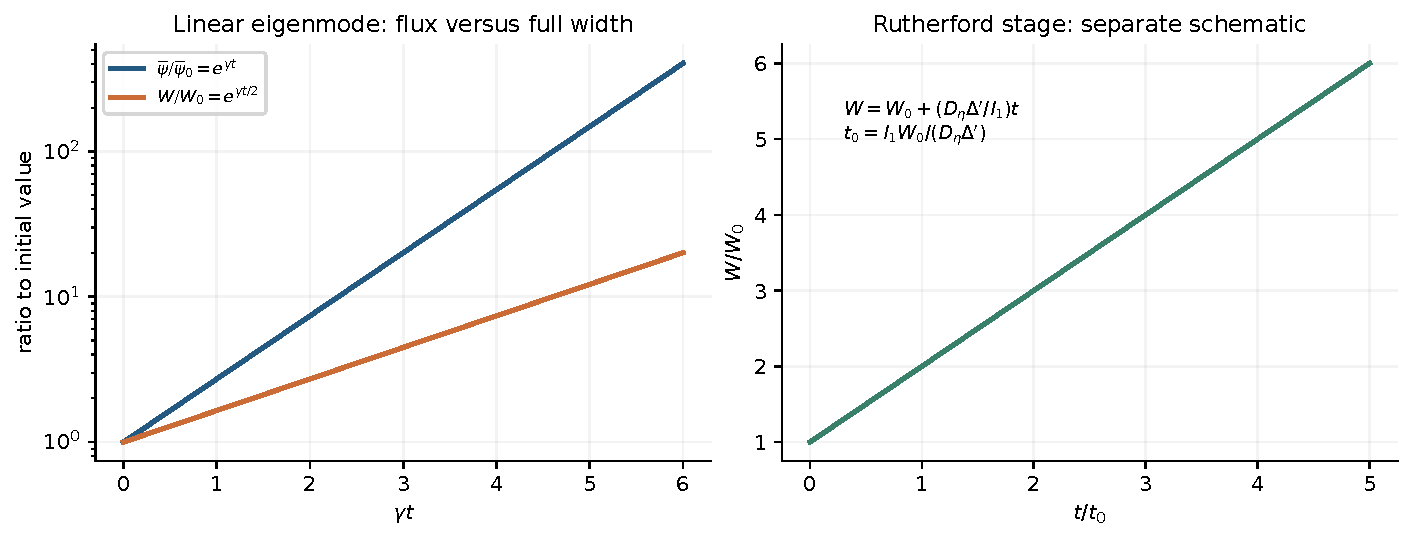
\includegraphics[width=\textwidth]{figures/tm_growth_observables.pdf}
\caption{不同观测量的增长曲线：在线性阶段，磁通幅和岛宽的半对数斜率分别为$\gamma$与$\gamma/2$。独立面板展示常$\Delta'$下Rutherford岛宽线性增长。各面板为解析教学曲线，没有强行拼成一条完整非线性时间轨道，也不是实验数据。}
\label{tm:fig:time}
\end{figure}

\section{一条长电流片为什么可能长出很多岛}
前面$a$是固定平衡片半厚。现在考虑长度尺度为$L$、厚度由Sweet--Parker平衡给出的长薄片。令
\begin{equation}
 S_L=\frac{LV_A}{D_\eta},\qquad \frac aL\sim S_L^{-1/2}.
\end{equation}
这里$L$的半长/全长约定会影响系数，本节只推导幂指数。最重要的一步是把\emph{局地片厚归一化}与\emph{全局长度归一化}分开：
\begin{equation}
 S_a=\frac{aV_A}{D_\eta}=\frac aL S_L\sim S_L^{1/2},
 \qquad \frac{\tau_{A,L}}{\tau_{A,a}}=\frac La\sim S_L^{1/2}.
\end{equation}
将式\eqref{tm:fastest}逐项换单位：
\begin{align}
 \gamma_{\max}\tau_{A,L}
 &=\left(\gamma_{\max}\tau_{A,a}\right)\frac La
 \sim S_a^{-1/2}S_L^{1/2}
 \sim\boxed{S_L^{1/4}},\label{tm:plasmoidgamma}\\
 k_{\max}L&=(k_{\max}a)\frac La
 \sim S_a^{-1/4}S_L^{1/2}
 \sim\boxed{S_L^{3/8}},\label{tm:plasmoidk}\\
 \frac{\delta_{\rm in}}L&=\frac{\delta_{\rm in}}a\frac aL
 \sim S_a^{-1/4}S_L^{-1/2}
 \sim\boxed{S_L^{-5/8}}.\label{tm:plasmoidwidth}
\end{align}
局地$\gamma\tau_{A,a}\sim S_L^{-1/4}\ll1$，却有全局$\gamma\tau_{A,L}\sim S_L^{1/4}\gg1$。两者不矛盾：厚度$a$远小于长度$L$，对应的Alfv\'en时间不同。所谓快于全局Alfv\'en时间，不意味着信号在局地超过光速或立即跨越整个系统。

以上重新获得plasmoid不稳定性的核心标度。Loureiro等的原始分析进一步采用带出流的薄片平衡并检查相应排序；这里的Harris式推导用于说明标度机制，不冒充与其平衡完全一致的数值系数。\citep{TMLoureiro2007}

\paragraph{再算一组长度、时间与岛数。}
取自设$L=10\,\mathrm m$、$V_A=10^5\,\mathrm{m/s}$、$D_\eta=0.01\,\mathrm{m^2/s}$，则$S_L=10^8$，
\begin{align}
 a&\sim10\times10^{-4}=1.0\,\mathrm{mm},&
 S_a&\sim10^4,\\
 \tau_{A,L}&=10^{-4}\,\mathrm s,&
 \gamma_{\max}&\sim10^2/\tau_{A,L}=10^6\,\mathrm{s^{-1}},\\
 \delta_{\rm in}&\sim10(10^8)^{-5/8}=10^{-4}\,\mathrm m,&
 k_{\max}L&\sim(10^8)^{3/8}=10^3.
\end{align}
因此局地增长时间约$1\,\mu\mathrm s$，内层约$0.1$毫米。若为长度$L$的周期示意区间，几何可容纳的波周期数约$k_{\max}L/(2\pi)\sim159$；开放出流片的最终可见岛数还会受排出、并合、噪声和非线性影响，不能把159当作实验应该拍到的精确岛数。

还必须检查出流。若出流率$V_A/L$与$\gamma$同阶或更大，小扰动可能在长成明显磁岛前已被排走；静态无限长片的本征增长率不能直接等同于有限寿命片的破碎时刻。经常出现的临界$S$量级也依赖噪声、边界、黏性和片形成历史，不是由式\eqref{tm:plasmoidgamma}单独推出的普适整数。

\section{电流片逐渐变薄：并不一定先形成稳态Sweet--Parker片}
设形成中的片有$a/L\sim S_L^{-\alpha}$。局地$S_a\sim S_L^{1-\alpha}$，因此
\begin{equation}
 \gamma_{\max}\tau_{A,L}
 \sim S_a^{-1/2}\frac La
 \sim S_L^{-(1-\alpha)/2+\alpha}
 =S_L^{(3\alpha-1)/2}.
\end{equation}
取$\alpha=1/3$可得到$\gamma_{\max}\tau_{A,L}\sim O(1)$。这是常被称为“理想撕裂”厚度标度的简单来源；名称指\emph{全局增长时间趋于Alfv\'en量级}，并不意味着内层变成严格理想、完全没有磁冻结破坏机制。若真的令所有非理想项为零且要求光滑解，不能借这个名称让磁力线凭空改变拓扑。

这个算式仍是假定背景片形状可用准静态序列描述。真正何时破碎还要比较片变薄率、种子谱与累计放大
\begin{equation}
 \ln\frac{\widetilde\psi(t)}{\widetilde\psi(t_0)}
 =\int_{t_0}^{t}\gamma[a(t'),k,\ldots]\,\dd t'.
\end{equation}
瞬时$\gamma$很大不等于已经积累足够增长；反之，较小增长率也可在长时间后产生显著磁岛。这里不代替完整动态形成理论。

\section{经典电阻理论何时需要交给双流体或动理学}
经典FKR推导中流体具有共同速度，并用$\eta\J$破坏磁冻结。真实电子--离子等离子体的欧姆律还可能包含
\begin{equation}
 \E+\vct u_i\times\B
 =\frac{\J\times\B}{en}
 -\frac{\nabla\cdot\vct P_e}{en}
 -\frac{m_e}{e}\left(\partial_t+\vct u_e\cdot\nabla\right)\vct u_e
 +\eta\J,\qquad
 \vct u_e=\vct u_i-\frac{\J}{en}.
\end{equation}
这里$n$为准中性数密度，$e>0$，$\vct P_e$为电子压力张量。它们各自需要不同变量与闭合。加入Hall项后磁场可相对离子运动，电子惯性和压力张量又改变更内层的平衡；不能只把FKR公式里的$\eta$换成一个“有效Hall电阻”。

常见微观长度为
\begin{equation}
 d_i=\sqrt{\frac{m_i}{\mu_0ne^2}},\quad
 d_e=\sqrt{\frac{m_e}{\mu_0ne^2}},\quad
 \rho_s=\frac{\sqrt{eT_e/m_i}}{\Omega_{ci}},\quad
 \Omega_{ci}=\frac{eB}{m_i}.
\end{equation}
此式$T_e$以eV表示，所以$eT_e$具有能量单位。$d_i$与离子--电子漂移尺度相关；强导场中的$\rho_s$、压力和声响应也可能进入排序。实际阈值应来自线性化后的各项比较，而不是任取一个长度就宣布所有情况下的转变点。\citep{TMHall2011}

\paragraph{把前面的数学算例放进真实参数会发生什么。}
以氢离子、$n=10^{20}\,\mathrm{m^{-3}}$计算，取$m_i=1.673\times10^{-27}\,\mathrm{kg}$、$e=1.602\times10^{-19}\,\mathrm C$，得到
\begin{align}
 d_i&=\sqrt{\frac{1.673\times10^{-27}}
 {(1.2566\times10^{-6})(10^{20})(1.602\times10^{-19})^2}}
 =2.28\times10^{-2}\,\mathrm m,\\
 d_e&=d_i\sqrt{m_e/m_i}=5.31\times10^{-4}\,\mathrm m.
\end{align}
第\ref{tm:matching}章算例的$\delta_*=5.63\times10^{-4}\,\mathrm m$于是满足
\begin{equation}
 d_i/\delta_*=40.5,\qquad d_e/\delta_*=0.94.
\end{equation}
这些长度比是重新检查双流体排序的警报，不能单独证明每一个电子惯性项都占主导。尤其是电子速度含$-\J/(en)$，其时间导数给广义欧姆定律带来的电流惯性项约为
\begin{equation}
 E_{\text{电子时间惯性}}
 \sim\frac{m_e}{ne^2}\gamma J
 =\mu_0d_e^2\gamma J.
\end{equation}
与电阻项$E_\eta=\eta J=\mu_0D_\eta J$比较，得到
\begin{equation}
 \frac{E_{\text{电子时间惯性}}}{E_\eta}
 \sim\frac{\gamma d_e^2}{D_\eta}
 =\frac{(250.97)(5.3146\times10^{-4})^2}{0.01}
 =7.09\times10^{-3}.
\end{equation}
所以即使$d_e/\delta_*\simeq0.94$，在这组增长率下，电子时间惯性仍只有电阻项的约$0.7\%$。原因是常磁通层内$\Psi''\sim\Delta'\Psi/\delta_*$，并非$\Psi/\delta_*^2$；仅按长度替换导数会丢失这个排序。上述比较只检查电子时间惯性，未检查电子对流惯性、压力及Hall耦合。较大的$d_i/\delta_*$仍提示必须把Hall响应代回线性方程比较，不能据经典FKR的内部排序就宣布它适用于这组实际等离子体。

若依然指定$V_A=10^5\,\mathrm{m/s}$，相应重联场为
$B_0=V_A\sqrt{\mu_0m_in}=0.0458\,\mathrm T$；它不会改变上述$d_i,d_e$。这正是要同时查长度、时间和各项实际幅值的原因。

此外需检查碰撞：局地电阻与流体热闭合通常要求相关时间和空间尺度上有足够的碰撞松弛。$\nu_{ei}\gg\gamma$是必要比较之一，却不能代替平行平均自由程$\lambda_{\rm mfp}$与实际梯度长度的比较。薄层里的$k_\parallel$接近共振而沿场连接长度很长，不能简单用$\delta$替代所有方向的梯度尺度。若压力张量、热流或粒子共振重要，应回到双流体矩方程或动理学方程，而不是对经典公式作无依据外推。

\section{与托卡马克撕裂模的桥梁：先认出共振条件}
在大长径比圆柱近似中，令$r,\theta,\zeta$分别为径向、极向和环向角，主半径为$R$。扰动相位写成$m\theta-n\zeta$，平衡场有$B_\theta,B_\zeta$。沿场导数作用于扰动给
\begin{equation}
 \B_0\cdot\nabla e^{i(m\theta-n\zeta)}
 =i\left(\frac{mB_\theta}{r}-\frac{nB_\zeta}{R}\right)
 e^{i(m\theta-n\zeta)}.
\end{equation}
定义安全因子$q(r)=rB_\zeta/(RB_\theta)$，括号可写为
\begin{equation}
 \frac{B_\theta}{r}[m-nq(r)].
\end{equation}
因此共振面满足$q(r_s)=m/n$。例如$2/1$模的共振面在$q=2$处；这与slab的$\vct k\cdot\B_0=0$是同一个逻辑。$q'(r_s)$决定局地磁剪切，与slab的$B'_0$相联系。

但圆柱/环形的外区方程、壁面响应和压力曲率不同，不能把Harris片$\Delta'$原封不动搬进托卡马克。新经典撕裂模还涉及磁岛内压强展平引起的bootstrap电流缺失及有限种子阈值；它可以在经典$\Delta'<0$时受到驱动。实验章将把这些结果与本章经典Rutherford方程分别对照，避免把所有“有磁岛”的信号都叫作同一个FKR验证。

\section{把整条推导链用自己的话串起来}
平衡磁场和电流给出自由能与磁剪切；边界和平衡共同决定外区解及$\Delta'$。共振面附近，理想冻结关系要求的流动奇异，迫使电阻与惯性进入一个很薄的层。层内电流的积分必须补上外区斜率差，这个匹配条件选择$\gamma$和$\delta$。常磁通与大$\Delta'$采用不同二阶导数量级，因此给出不同指数。磁岛宽度超过线性层后，非线性改变平流与电流分布；弱驱动小岛可进入磁面近似平衡的Rutherford增长。片若足够细长，会有许多沿片波长同时增长；继续变薄后又可能进入双流体或动理学尺度。

这条链中的每一箭头都有假设。真正掌握理论，意味着面对新参数时能够列出这些假设、算出各项比值、发现哪一步先失效，并据此选择新的方程；不是只会背诵一个$\eta^{3/5}$。

\chapter{从磁岛图像到实验检验：实验究竟测到了什么}
\label{tm:chap:experiments}

\section{先把三个不同的问题分开}

理论推导得到的是一个本征模：给定平衡、边界条件和闭合，求扰动的空间结构及增长率。实验仪器直接给出的却可能是线圈电压、辐射强度或粒子照相。要把两者连起来，需要经过诊断标定、几何重建和模型比较。以下三个命题的证据强度不同。

\begin{enumerate}
  \item \textbf{存在磁岛。}需要看到闭合的扰动磁通面、O 点与 X 点，或多个相互支持的间接信号。这回答拓扑问题。
  \item \textbf{磁岛由某种撕裂不稳定性产生。}还要识别自由能、背景演化、种子扰动和可能的外部强迫。已有磁岛也可能是外部扰动驱动的。
  \item \textbf{某个具体增长率公式被检验。}应测量平衡、波数、耗散、线性区间的扰动幅度以及不确定度，然后比较公式。看到一串岛，尚不等于测得了 FKR 的 $S_a^{-3/5}$ 标度。
\end{enumerate}

特别要区分\emph{随时间增大}和\emph{线性本征模的指数增长}。若电流片在观察期间持续变薄，$a(t)$、$\Delta'(t)$、$S_a(t)$ 同时改变，用一条固定平衡的 $e^{\gamma t}$ 拟合就可能失去意义。若岛已进入 Rutherford 阶段，$W$ 可以近似随时间线性变化，但这不是“线性扰动理论阶段”：前一个“线性”描述曲线形状，后一个“线性”描述方程对扰动幅度的截断。

本章选择三类原始实验：托卡马克中的新经典撕裂模控制、专门重联装置中的碰撞性双流体电流片，以及激光产生的快速演化高 $\beta$ 电流片。它们检验理论的不同部分，不能排成一条由低到高的“模型正确率”。文中重新绘制的图全部为教学示意或解析曲线，\textbf{没有把自设数据画成实验结果}。原论文的图号用于指导读者回到原始证据。

\section{从平板共振面走向托卡马克有理面}

\subsection{为什么会出现 \texorpdfstring{$q=m/n$}{q=m/n}}

在大环径、近圆截面的近似下，以 $r$ 表示小半径，$R$ 表示大半径，$\theta$ 为极向角，$\zeta$ 为环向角。设一个螺旋扰动的相位为
\begin{equation}
 \alpha=m\theta-n\zeta-\omega t,
 \qquad m,n\in\mathbb Z.
 \label{tm:helical_phase}
\end{equation}
整数性来自角度增加 $2\pi$ 后物理量必须单值。在圆柱近似下，
\begin{equation}
 \B\cdot\nabla\alpha
 =\frac{mB_\theta}{r}-\frac{nB_\zeta}{R}.
\end{equation}
定义安全因子
\begin{equation}
 q(r)\simeq\frac{rB_\zeta}{RB_\theta},
 \qquad
 k_\parallel\equiv\frac{\B\cdot\nabla\alpha}{B}
 =\frac{B_\zeta}{RB}\left(\frac{m}{q}-n\right).
 \label{tm:q_resonance}
\end{equation}
当 $q(r_s)=m/n$ 时，$k_\parallel(r_s)=0$。这表示沿平衡磁力线走动时，该扰动的螺旋相位在共振面上不变。它是前面平板模型 $\vct{k}\cdot\B_0=0$ 的环形对应物。\emph{并不是磁场本身变成零}：托卡马克通常有很强的环向磁场。对真实成形平衡，$q$ 通过磁力线的一周积分定义，仍有有理面共振；上述简单局地表达式只用于建立直观。

写 $x=r-r_s$，在 $|x|$ 足够小时作泰勒展开，
\begin{equation}
 k_\parallel(x)\simeq k_\parallel'(r_s)x,
 \qquad
 k_\parallel'(r_s)=-\frac{B_\zeta}{RB}\frac{m q'(r_s)}{q_s^2}.
 \label{tm:kpar_shear}
\end{equation}
因为括号 $m/q-n$ 在 $r_s$ 恰好为零，对前因子求导所得的项消失。$q'$ 所表达的磁剪切，正是局地 $B_y\simeq B'x$ 中 $B'$ 的对应物。

\begin{figure}[htbp]
 \centering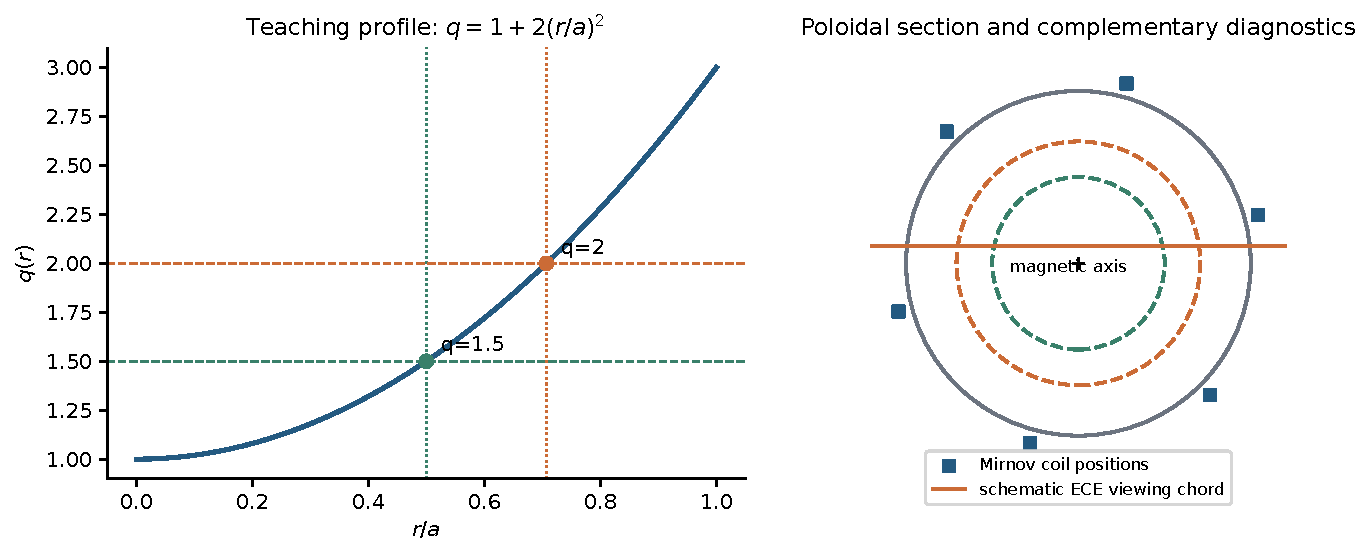
\includegraphics[width=0.94\textwidth]{figures/tm_rational_diagnostics.pdf}
 \caption{自设的托卡马克教学几何。左：$q=1+2(r/a)^2$ 的 $q=3/2$ 与 $q=2$ 有理面。右：圆截面磁面、外部 Mirnov 线圈与一条 ECE 观测弦的示意。此图不对应 DIII-D 的实际成形平衡，也没有模拟辐射传输。}
 \label{tm:fig:rational}
\end{figure}

\subsection{“一个 \texorpdfstring{$m/n=2/1$}{m/n=2/1} 模”意味着什么}

固定 $\zeta$，相位随 $\theta$ 变化两周；固定 $\theta$，随 $\zeta$ 变化一周。这并不意味着任何一张相机照片都必然显示两个清晰孤立的圆斑。视线积分、岛的相位、磁面形状和诊断响应会改变图像。实际模式识别通常同时使用多个线圈的相位、平衡重建的 $q$ 剖面以及内部温度扰动。

\section{从仪器信号重建岛：一步一步解释}

\subsection{Mirnov 线圈首先测到的是电压}

小线圈包围面积 $A$，匝数 $N$，若磁场在其面积内近似均匀，法拉第定律给出
\begin{equation}
 V(t)=-N A_{\rm eff}\frac{\dd\delta B_{\perp}}{\dd t}.
 \label{tm:mirnov_voltage}
\end{equation}
这里 $\perp$ 是线圈法向，而非必然等于平衡场的垂直方向；有效面积还取决于方向和标定。测得电压后，通过传递函数校正和时间积分才得到磁扰动。积分常数、低频漂移、导体壁屏蔽及线缆相位都应处理。

若单一模式近似为
\begin{equation}
 \delta B_j(t)=A(t)\cos\!\left(m\theta_j-n\zeta_j-\omega t+\alpha_0\right),
 \label{tm:mirnov_B}
\end{equation}
同一时刻两个探头的相位差满足
\begin{equation}
 \Delta\alpha=m\Delta\theta-n\Delta\zeta\pmod {2\pi}.
 \label{tm:phase_difference}
\end{equation}
知道探头位置后，拟合整数 $m,n$。只有一个极向阵列无法独立确定环向模数；稀疏阵列还会产生相位混叠。实际需要多个位置、频带相干性和连续相位展开，而不是用两点决定所有模式。

\begin{figure}[htbp]
 \centering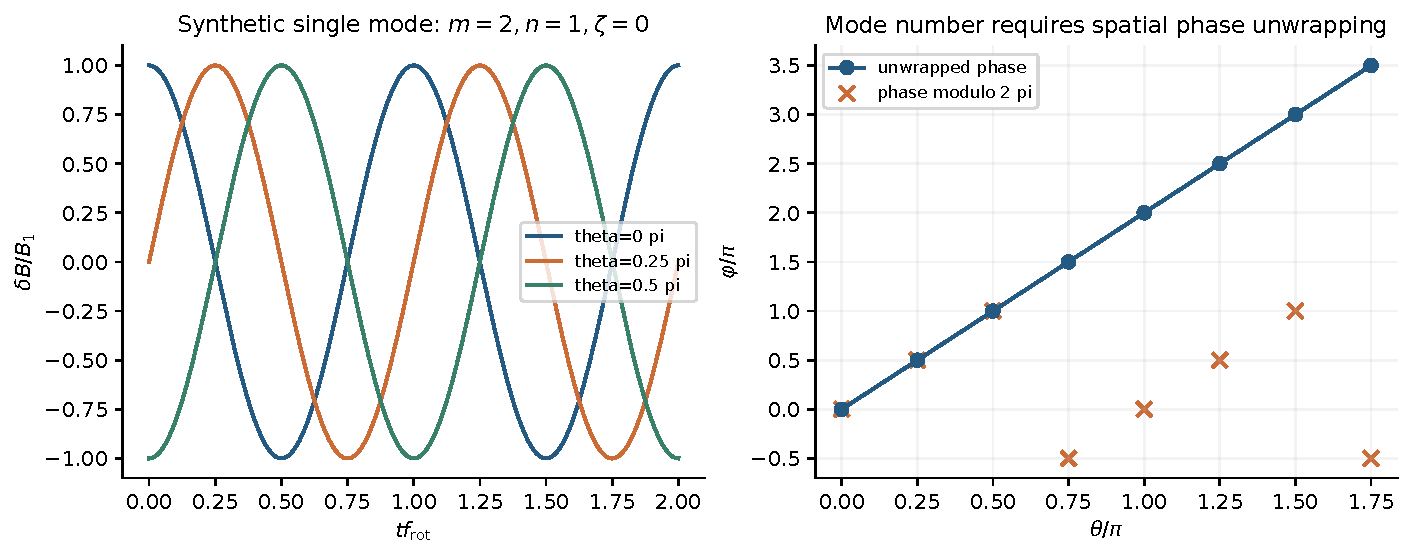
\includegraphics[width=0.94\textwidth]{figures/tm_mirnov_phase.pdf}
 \caption{合成的 $m=2,n=1$ 磁场信号。左图三个极向位置的时间相位不同；右图展示相位的 $2\pi$ 包裹与展开。画的是已还原的 $\delta B$，不是原始线圈电压；没有噪声、壁响应或多模叠加，不是实验数据。}
 \label{tm:fig:mirnov}
\end{figure}

对 $A(t)=A_0e^{\gamma t}$ 求导，电压含有两个分量：
\begin{equation}
 V=-NA_{\rm eff}A(t)\,[\gamma\cos\alpha+\omega\sin\alpha].
\end{equation}
电压包络为 $NA_{\rm eff}A\sqrt{\gamma^2+\omega^2}$。当 $|\omega|\gg\gamma$，电压幅度主要正比于 $|\omega|A$。因此模式旋转减慢时，电压可降低而磁扰动并未同比降低；完全锁定且不再增长的岛甚至不产生持续感应电压。要宣称“岛消失”，不能只看到某个交流频带信号变小，还应结合低频/静态磁测量、温度结构或其他诊断。

\subsection{为什么磁岛会使温度变平}

沿磁场的电子热传导通常远强于跨场热传导。一个最简输运模型是
\begin{equation}
 \frac{\partial T_e}{\partial t}
 =\chi_\parallel\nabla_\parallel^2T_e+
   \chi_\perp\nabla_\perp^2T_e+Q_T,
 \label{tm:anisotropic_heat}
\end{equation}
其中 $\chi$ 为热扩散率（$\mathrm{m^2\,s^{-1}}$），$Q_T$ 是换算成温度变化率的源项。这是教学闭合，实际热通量还可能非局地且包含湍流。

磁岛形成后，一条闭合的螺旋磁力线访问原本不同半径的位置。沿线传热把这些位置的温差拉小，岛内温度便倾向于在螺旋磁通面上近似相等。穿过 O 点的径向剖面最容易出现平坦区；穿过 X 点或分离界附近则不同。岛旋转经过固定探头时，这种空间结构变成周期信号，跨越共振面的若干温度扰动通道还可能出现相位反转。

“出现岛就立即完全平坦”也不准确。扩散时间分别约为 $\tau_\parallel\sim L_\parallel^2/\chi_\parallel$ 和 $\tau_\perp\sim W^2/\chi_\perp$。小岛附近有效平行连接长度大，平行均温可能赶不上跨场补给及源项，形成有限宽度阈值。故没有显著温度平坦区，并不单独排除很小的磁岛；平坦区的宽度也不能未经诊断卷积就直接当成 $W$。

\subsection{ECE、软 X 射线和平衡重建各补哪一块信息}

电子回旋辐射（ECE）的观测频率与局地磁场有关：在最简非相对论近似下，
\begin{equation}
 f\simeq s f_{ce}=s\frac{eB}{2\pi m_e},\qquad s=1,2,\ldots .
\end{equation}
若等离子体在该频带光学厚、电子接近热分布，并正确处理传播与相对论展宽，亮温可以用来推断电子温度。由于 $B$ 随位置变化，多频通道近似对应不同径向位置，从而看到岛导致的温度结构。频率通道的有限宽度意味着有限空间分辨率；非热电子、光学薄区域或反射会破坏简单的“亮温等于 $T_e$”。

软 X 射线（SXR）的单条观测弦更接近
\begin{equation}
 I_{\rm SXR}\propto\int_{\rm chord} n_e^2\,Lambda(T_e,Z_{\rm eff},\ldots)\,\dd l,
\end{equation}
其中 $\Lambda$ 包括辐射过程、杂质和探测器谱响应。它是视线积分，并非单点温度计。多弦层析及相位分析能识别旋转结构，但密度、温度与杂质变化可能互相混淆。磁测量给模数，ECE/SXR 给内部结构，动理学剖面和平衡重建给有理面位置，组合证据更有说服力。运动斯塔克效应（MSE）可提供磁场方向约束，帮助平衡重建推断 $q(r)$；$q$ 并非由一支 Mirnov 线圈直接读出。

\section{经典、NTM、强迫重联和锯齿：相似图像不等于相同驱动}

\subsection{新经典撕裂模的正反馈}

在环形装置中，粒子会受到磁场强度沿磁力线变化的影响；一部分粒子被磁镜俘获。碰撞、俘获与通过粒子的输运耦合，使压力梯度能够驱动自举电流（bootstrap current）。这里的“新经典”指把环形几何及俘获粒子纳入碰撞输运理论，不是“新提出的经典撕裂模”。自举电流的系数需要更完整的新经典输运计算，不能从平板不可压缩 MHD 自动推出。

对常见的托卡马克参数，岛内压力平坦化会降低本来由压力梯度维持的局地自举电流。这个缺额具有与岛同相的螺旋结构，进一步加强岛。这就形成
\begin{equation}
 \text{有限种子岛}\ \longrightarrow\ \text{压力平坦化}
 \ \longrightarrow\ \text{自举电流缺额}
 \ \longrightarrow\ \text{岛继续增大}.
\end{equation}
即使经典项 $\Delta'_{\rm class}<0$，附加驱动也可能使有限岛增长。小岛时的有限平坦化、极化电流和其他效应决定是否有阈值；因此 NTM 的有限幅度触发，与经典 FKR 从任意小扰动出发的线性不稳定性不是同一个问题。

\begin{figure}[htbp]
 \centering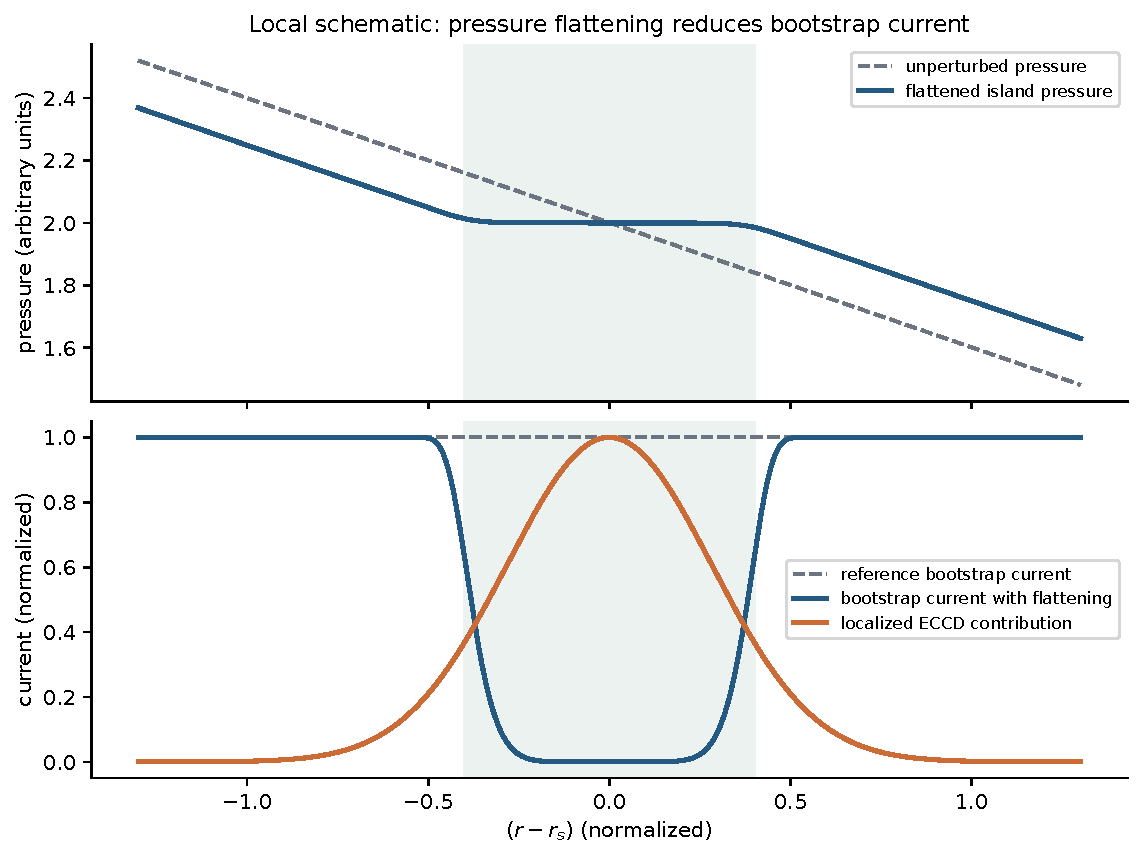
\includegraphics[width=0.94\textwidth]{figures/tm_bootstrap.pdf}
 \caption{自设的 NTM 教学图：压力平坦化、相应的自举电流缺额，以及在同一位置补充的局地 ECCD。曲线由脚本给定解析轮廓，仅解释反馈方向；不是 DIII-D 数据，也不是新经典输运方程的数值解。实际电流和驱动还依赖螺旋相位、岛宽、沉积宽度与偏心量。}
 \label{tm:fig:bootstrap}
\end{figure}

为保持量纲清楚，可把\emph{修正 Rutherford 方程的组织形式}写为
\begin{equation}
 \frac{I_1}{D_\eta}\frac{\dd W}{\dd t}
 =\Delta'_{\rm class}
 +\Delta'_{\rm BS}(W)
 +\Delta'_{\rm pol}(W)
 +\Delta'_{\rm CD}(W,\Delta r,w_{\rm CD})+\cdots .
 \label{tm:mre_structure}
\end{equation}
这里各个有效 $\Delta'$ 的单位都是 $\mathrm{m^{-1}}$；$\Delta r$ 为电流驱动相对有理面的偏心量，$w_{\rm CD}$ 为驱动分布宽度。$I_1\simeq0.823$ 对应前文特定全宽、局地电阻模型的归一化；真实环形模型经常吸收系数并使用不同长度。式\eqref{tm:mre_structure}是分类表达，\emph{不是给所有装置通用的精确闭合公式}。自举、极化、有限输运和电流驱动项的系数与符号应从所选模型求得，不能把平板系数与另一篇论文的宽度定义混用。

电子回旋电流驱动（ECCD）利用波对电子速度分布的非对称作用来驱动电流。若在岛的合适位置补回缺失电流，可产生稳定作用。它既需要足够总功率，也需要合适位置和窄的沉积轮廓：同样的总电流均摊到太宽区域，有效螺旋电流分量就小。

\subsection{其他几种容易混淆的情形}

\begin{itemize}
 \item \textbf{强迫重联：}外部共振磁场或边界运动提供扰动。一个经典线性稳定、$\Delta'<0$ 的平衡也可能形成有限磁岛；研究的是响应、穿透与重联过程，不能仅凭岛存在宣布自发线性不稳定。
 \item \textbf{锯齿：}托卡马克核心温度周期性缓慢上升、快速崩塌，常涉及 $q\simeq1$ 附近的 $m=n=1$ 内扭曲及重联。它包含重联物理，却不等于本讲义的静态 Harris 平板 FKR 问题；锯齿还可为别的有理面上的 NTM 提供种子。
 \item \textbf{磁岛链/plasmoid：}这是结构名称。可能来自电阻性撕裂、Hall/电子尺度撕裂、随时间变薄电流片的多模过程或其他动力学。需要尺度排序和演化证据识别具体机制。
\end{itemize}

\section{实验一：DIII-D 对 NTM 的定点电流驱动控制}
\label{tm:sec:diiid}

本节采用可完整取得的 \citet{TMPetty2003} 原始技术报告 GA--A24317，版本为 2003 年射频会议预印本。PDF 共 7 页，其中正文为报告页 1--4。\textbf{它不是对随后正式期刊版本的逐页核读替代品。}图 1 给出成形平衡、回旋共振面、波轨迹、ECE 与 MSE 几何；图 2--4 分别提供控制时间轨迹、位置扫描和模型比较。

\paragraph{装置、驱动和测量。}
DIII-D 中的 $m/n=2/1$ NTM 位于 $q=2$ 面。实验使用最高合计 $2.7\,\mathrm{MW}$ 的吸收 ECCD 功率，回旋管频率 $110\,\mathrm{GHz}$。文中的约 $40\,\mathrm{kA}$ 驱动电流是 CQL3D 计算结果，不是独立的直接电流探针测量。外部 Mirnov 信号跟踪 $n=1$ 磁扰动；$q=2$ 位置来自平衡重建，ECCD 位置来自射线追踪。

\paragraph{关键比较。}
原文图 2 对比完全和部分抑制的放电；图 3 扫描环向磁场，使 ECCD 沉积经过共振位置，磁扰动在两者对齐附近最小。完全抑制案例的反馈调整约为 $0.01\,\mathrm T$，相当于中平面沉积位置移动约 $0.9\,\mathrm{cm}$。这说明“放进功率”之外，\emph{把电流驱动放在正确位置}是关键变量。

\paragraph{模型比较到什么程度。}
图 4 用修正 Rutherford 模型比较\emph{部分抑制扫描}中最小岛宽：测得约 $8\,\mathrm{cm}$，由沉积全半高宽约 $3.3\,\mathrm{cm}$ 的模型匹配；射线追踪给出的宽度为 $2.6\,\mathrm{cm}$，允许的比较范围约 $2.6$--$3.9\,\mathrm{cm}$。不要把这里的 $8\,\mathrm{cm}$ 误写成完全抑制案例的初始岛宽。图中理论误差条包含回旋管功率的 $10\%$ 不确定性。

\paragraph{可以得出与不能得出的结论。}
该实验直接支持局地电流驱动能够控制 NTM，以及控制对共振位置的敏感性。它不是经典 FKR 线性增长率的检验；$q$ 位置、沉积轮廓和驱动电流包含反演或模型。用岛宽约束沉积宽度时，参数是经模型推断的，不应又把同一个岛宽当作完全独立的预测成功。放电还通过中性束反馈调节能量和 $\beta$，评估控制效果要同时看这些轨迹。上述结论均对应原文图 1--4 及其说明。\citep{TMPetty2003}

\section{实验二：MRX 的碰撞性双流体电流片和岛链}
\label{tm:sec:mrx}

\citet{TMJaraAlmonte2016} 在磁重联实验装置 MRX 的氩等离子体中观测到岛链。所读作者稿共 5 页，对应 PRL 117, 095001。它特别适合纠正“Hall 效应出现就一定无碰撞”的误解。

\paragraph{参数与尺度。}
上游典型 $n_e\simeq5\times10^{19}\,\mathrm{m^{-3}}$、$T_e\simeq3\,\mathrm{eV}$，片内约 $2\times10^{20}\,\mathrm{m^{-3}}$、$4\,\mathrm{eV}$。原文代表性排序为
\begin{equation}
 d_e\sim0.5\,\mathrm{mm}
 <\lambda_{\rm mfp}\sim2\,\mathrm{mm}
 <\delta\sim9\,\mathrm{mm}
 \ll d_i\sim200\,\mathrm{mm},
 \label{tm:mrx_scales}
\end{equation}
其中 $\delta$ 是电流片半厚度。离子不能在片尺度上简单地与电子共同运动，但片厚又比电子惯性尺度和电子平均自由程大；因此 Hall 物理与碰撞性电阻可以同时重要。

\paragraph{怎样认出岛。}
约 400 个拾取线圈测量三分量磁场，最好采样间距跨片约 $6\,\mathrm{mm}$、沿片约 $3\,\mathrm{cm}$。原文图 2 展示重建磁通轮廓和法向磁场翻转；作者还用局部磁矢量的绕数识别 O/X 点，检查插值是否凭空产生小岛。原文坐标与本讲义不同：其径向跨片方向对应本讲义 $x$，出流方向对应 $y$，出平面电流方向对应 $z$，不能照搬下标。

\paragraph{统计结果与模型解释。}
图 3 比较平均岛数、长宽比与 Lundquist 数；研究包含约 200 次放电和 500 次形成事件。许多岛出现在 $S<100$ 的范围。图 4--5 将岛形成与重联率变化联系起来，超过四分之三事件的重联率增加，平均一个岛的形成对应约 $10\%$ 的归一化率增加；原文对率给出约 $10\%$ 的保守不确定性。这是事件统计，不表示每个岛都会精确产生同样增益。\citep{TMJaraAlmonte2016}

\paragraph{为何不能直接拿经典临界数判错。}
常被引用的 $S\sim10^4$ 是特定高 $S$ 电阻 MHD 电流片及其形成条件下的参考，不是“所有岛的普适门槛”。MRX 的 Hall 尺度、可压缩性、有限长宽比和持续驱动都影响稳定性。原文将结果解释为电阻性电子撕裂，同时明确指出，含实际密度、Hall 场和几何的二维线性比较仍不充分。$6\,\mathrm{mm}$ 的探头间距不能分辨 $0.5\,\mathrm{mm}$ 电子惯性层；观测到拓扑与 Hall 场，也不能单独给出所有电子解冻项的精确预算。图 3 的总体散布与均值误差是不同误差条，读图时亦应区分。\citep{TMJaraAlmonte2016}

\section{实验三：激光高 \texorpdfstring{$\beta$}{beta} 等离子体中的 plasmoid 证据}
\label{tm:sec:laser}

\citet{TMPearcy2024} 使用 OMEGA EP 激光驱动两个磁化等离子体泡碰撞。所读为作者机构公开的 PRL 132, 035101，7 页，包括方法附录；它把磁场照相、反演及有限时间分辨率的问题展示得很清楚。

\paragraph{如何产生和拍摄电流片。}
两个 $930\,\mathrm J$、$1\,\mathrm{ns}$ 的相互作用激光脉冲照射 CH 薄膜，产生膨胀磁化泡。质子照相利用质子穿过磁场时的偏转，把偏转映射为探测面上的通量明暗。不同能量的质子具有不同飞行时间，从同次实验得到多个时间切片。图 1 给出装置；图 2--3 比较质子图像与重建的磁场、磁通和电流；图 4 检查法向场的符号变化。

\paragraph{实测与反演量要分开。}
直接记录的是质子在胶片上的空间分布。路径积分磁场由反问题求得，再推断磁通岛和电流结构；局地 $B$ 还需要场区路径长度假设。文中典型 $B\sim40$--$70\,\mathrm T$、$\beta\sim10$，表 I 给出 $L\sim2000\,\mu\mathrm m$、电流片宽度 $20$--$60\,\mu\mathrm m$、$d_i\sim55\,\mu\mathrm m$、$d_e\sim1\,\mu\mathrm m$。这里实验电流宽度按电流轮廓全半高宽定义，不能当成前文 Harris 参数 $a$。

\paragraph{观察到了什么。}
重建磁通出现约 $100$--$200\,\mu\mathrm m$ 的岛结构；图 4 的场翻转提供进一步检验。图 5 的电流轮廓显示片宽变化；图 6 跟踪岛宽。中央和右侧岛在误差内没有可辨认增长；左侧结构的快速变宽受边缘流动和几何影响，作者没有把它直接当作线性撕裂增长率。\citep{TMPearcy2024}

\paragraph{限制决定了应如何解释。}
这是一张快速形成且持续受驱动的电流片，未必满足静态 Sweet--Parker 或 FKR 假设。反演涉及入射质子通量、轨迹映射、能量展宽和磁偏转主导的假设；测得的是沿视线积分量，没有同时的侧向三维重建。部分等离子体参数来自名义相同驱动条件下的另一组 Thomson 散射实验，并非所有量都在同一次照相放电里同时测得。它支持高 $\beta$ 重联中存在 plasmoid 及离子尺度附近的片结构，但不构成对某一普适 $\gamma(S)$ 的直接测量。下一章会算出：在其可用时间窗里，典型重联速度预期造成的岛宽变化完全可能低于空间分辨率。\citep{TMPearcy2024}

\section{把三个实验放回理论学习路线}

\begin{table}[htbp]
\centering\small
\begin{tabular}{p{0.16\textwidth}p{0.35\textwidth}p{0.36\textwidth}}
\toprule
研究 & 最直接支持的物理 & 没有由此自动完成的检验\\
\midrule
DIII-D NTM & 局地电流驱动及对齐可抑制有限岛；修正 Rutherford 模型有可检验的控制含义 & 经典 FKR 线性指数和完整新经典闭合的独立验证\\[3pt]
MRX 岛链 & 碰撞性电阻与双流体尺度可共存；磁拓扑与重联率有统计联系 & 实际二维平衡的完整本征值问题、每个电子解冻项和三维效应\\[3pt]
OMEGA EP & 快速演化高 $\beta$ 电流片中磁岛的成像证据 & 在分辨率不足的短窗内准确测得线性增长率；排除所有三维结构\\
\bottomrule
\end{tabular}
\caption{按原始论文证据范围作出的教学比较。各行的限制不否定实验结果，而是说明结果实际约束了理论的哪一部分。}
\label{tm:tab:experiments}
\end{table}

以后阅读一篇撕裂模实验论文，可以依次检查：扰动究竟是自发还是外加；模数及共振面如何确定；幅度是磁通、磁场、岛宽还是线圈电压；背景是否近似静态；岛宽定义和时间区间是否与理论一致；测量误差能否区分候选模型。这样才能从“图像很像”推进到“某个定量理论受到约束”。本讲义的源文件同时保存原文版本、阅读范围和图号，便于逐项回查，而没有将候选下载量改写成全库全文核读数量。

\chapter{把诊断、尺度和误差算到底}
\label{tm:chap:worked}

本章每个算例都给出输入、代入和判断。前三例采用自设教学参数，后面几例明确指出哪些输入摘自实验论文、哪些是为说明方法另加的近似。它们不是对原始实验数据的重新拟合。

\section{算例一：法向磁扰动怎样换成磁岛全宽}

取局地平衡和单一扰动
\begin{equation}
 \psi(x,y)=\frac{B'x^2}{2}+\widetilde\psi\cos ky,
 \qquad B'=2\,\mathrm{T\,m^{-1}},\quad k=20\,\mathrm{m^{-1}}.
\end{equation}
按本讲义约定 $\B=\widehat{\vct z}\times\nabla\psi$，法向分量为
\begin{equation}
 \delta B_x=-\partial_y\psi=k\widetilde\psi\sin ky.
\end{equation}
假设在有理面附近测得该单模法向场峰值 $b_x=0.20\,\mathrm{mT}$，则
\begin{equation}
 \widetilde\psi=\frac{b_x}{k}
 =\frac{2.0\times10^{-4}\,\mathrm T}{20\,\mathrm{m^{-1}}}
 =1.0\times10^{-5}\,\mathrm{T\,m}.
\end{equation}
量纲检查：二维磁通函数是 $\mathrm{T\,m}$，不是总磁通 $\mathrm{Wb}$，因为我们没有再乘出平面的长度。

X 点在 $(x,ky)=(0,0)$，分离界值为 $\psi_X=\widetilde\psi$。通过 O 点的径向截线是 $ky=\pi$。分离界与此截线相交时，
\begin{align}
 \frac{B'x^2}{2}-\widetilde\psi&=\widetilde\psi,\\
 x_{\rm sep}^2&=\frac{4\widetilde\psi}{B'},\\
 W=2|x_{\rm sep}|&=4\sqrt{\frac{\widetilde\psi}{B'}}
 =4\sqrt{\frac{10^{-5}}{2}}\,\mathrm m
 =8.94\,\mathrm{mm}.
 \label{tm:worked_width}
\end{align}
因此半宽为 $4.47\,\mathrm{mm}$。若误把 $W$ 写成半宽，后续涉及 $W^2$ 的项会差四倍。还要注意：这是\emph{有理面附近}的扰动幅度。壁上线圈的 $0.20\,\mathrm{mT}$ 不应直接代入；必须用外区本征函数、几何和壁响应把信号映射到共振面。

\section{算例二：有理面位置与平行相位尺度}

使用图\ref{tm:fig:rational}的自设剖面
\begin{equation}
 q(r)=1+2(r/a)^2,\qquad a=0.60\,\mathrm m,\qquad R=1.70\,\mathrm m.
\end{equation}
求 $2/1$ 面：$1+2(r_s/a)^2=2$，所以
\begin{equation}
 r_s=\frac{a}{\sqrt2}=0.4243\,\mathrm m.
\end{equation}
对 $3/2$ 面，$1+2(r_s/a)^2=1.5$，得到 $r_s=a/2=0.3000\,\mathrm m$。注意 $q=2$ 是磁力线绕行比，不是“半径等于 2”。

对于 $m=2,n=1$，在环向场占优的近似 $B_\zeta/B\simeq1$ 下，
\begin{align}
 q'(r_s)&=\frac{4r_s}{a^2}=4.714\,\mathrm{m^{-1}},\\
 k_\parallel'(r_s)&=-\frac{m q'}{R q_s^2}
 =-\frac{2\times4.714}{1.70\times4}
 =-1.386\,\mathrm{m^{-2}}.
\end{align}
离共振面向外 $x=1.0\,\mathrm{cm}$ 时，一阶估计给出
\begin{equation}
 k_\parallel\simeq-1.386\times0.010
 =-1.386\times10^{-2}\,\mathrm{m^{-1}},
 \qquad L_{\parallel,\alpha}\equiv\frac{2\pi}{|k_\parallel|}\simeq453\,\mathrm m.
\end{equation}
这是沿磁力线使\emph{扰动相位}改变 $2\pi$ 所需的局地长度，不是托卡马克的周长，也不是任何热粒子实际自由飞行的平均自由程。共振面上该相位长度发散，说明相位与平衡场线相锁；磁力线仍然在强磁场中延伸。

这一结果还解释了为什么小岛未必立即完全均温。仅作教学估计，取 $\chi_\parallel=10^8\,\mathrm{m^2/s}$、$\chi_\perp=1\,\mathrm{m^2/s}$，并\emph{暂用} $453\,\mathrm m$ 作为平行长度，则
\begin{equation}
 \tau_\parallel\sim\frac{453^2}{10^8}=2.05\,\mathrm{ms},
 \qquad
 \tau_\perp\sim\frac{(0.010)^2}{1}=0.10\,\mathrm{ms}.
\end{equation}
即使 $\chi_\parallel/\chi_\perp$ 很大，长连接距离也可能抵消它。这不是严格求出的磁岛平坦化阈值：实际岛内应沿岛磁场求连接长度和二维热输运。它说明比较扩散\emph{系数}之前，还必须比较扩散\emph{距离的平方}。

\section{算例三：从相位、幅度和电压得到不同物理量}

\subsection{先定模数，再定频率}

设一组理想合成信号满足式\eqref{tm:mirnov_B}。在相同环向角上，两个探头相差 $\Delta\theta=\pi/4$，展开后的相位差为 $\pi/2$。因此
\begin{equation}
 m=\frac{\Delta\alpha}{\Delta\theta}=2.
\end{equation}
另一对探头有相同极向角，$\Delta\zeta=\pi/3$，相位差为 $-\pi/3$，得到
\begin{equation}
 n=-\frac{\Delta\alpha}{\Delta\zeta}=1.
\end{equation}
如果只保留模 $2\pi$ 的相位而没有更多探头，第一对还可与其他整数相混淆。例如 $m=10$ 也给出 $10\pi/4=\pi/2+2\pi$。完整阵列及可信的模数范围才消除这种混叠。

周期测得 $T=0.10\,\mathrm{ms}$，故 $f=1/T=10\,\mathrm{kHz}$，$\omega=2\pi f=6.283\times10^4\,\mathrm{s^{-1}}$。频率表示模式旋转，不是增长率。旋转方向还需按照探头坐标和相位约定确定，单一功率谱峰不包含符号。

\subsection{磁场幅度增长四倍，岛宽只增长两倍}

假设已校正为磁场的单模包络在 $\Delta t=0.20\,\mathrm{ms}$ 内由 $0.10$ 增到 $0.40\,\mathrm{mT}$，背景及 $k$ 保持不变，并且这段确实处在线性阶段。由于 $b_x=k\widetilde\psi$，
\begin{equation}
 \gamma=\frac{\ln[b_x(t_2)/b_x(t_1)]}{t_2-t_1}
 =\frac{\ln4}{2.0\times10^{-4}}
 =6.931\times10^3\,\mathrm{s^{-1}},
 \quad \gamma^{-1}=144.3\,\mu\mathrm s.
\end{equation}
因 $W\propto\sqrt{\widetilde\psi}$，$W_2/W_1=\sqrt4=2$，岛宽对数斜率为
\begin{equation}
 \frac{\dd\ln W}{\dd t}=\frac\gamma2
 =3.466\times10^3\,\mathrm{s^{-1}}.
\end{equation}
把岛宽半对数图的斜率直接当 $\gamma$，会少一倍。

如果两个磁场幅度各有独立的 $5\%$ 标准不确定度，暂忽略时钟误差，对数误差传播给出
\begin{equation}
 \sigma_\gamma\simeq\frac{1}{\Delta t}
 \sqrt{\left(\frac{\sigma_{b_1}}{b_1}\right)^2+
       \left(\frac{\sigma_{b_2}}{b_2}\right)^2}
 =\frac{\sqrt{0.05^2+0.05^2}}{2\times10^{-4}}
 =354\,\mathrm{s^{-1}}.
\end{equation}
结果为 $(6.93\pm0.35)\times10^3\,\mathrm{s^{-1}}$，约 $5.1\%$。共同的乘法标定误差会在幅度比中抵消，不能总当作两次独立误差相加；平衡演化和噪声底则是另外的系统问题。

\subsection{为什么不能直接用线圈电压比}

若旋转频率从 $10$ 降到 $5\,\mathrm{kHz}$，真实磁场幅度同时增长四倍，则在 $|\omega|\gg\gamma$ 的近似下，电压只增长约
\begin{equation}
 \frac{|V_2|}{|V_1|}\simeq\frac{f_2b_2}{f_1b_1}=2.
\end{equation}
直接代入电压比会给出 $\ln2/\Delta t=3.466\times10^3\,\mathrm{s^{-1}}$，约少一半。若保留本例有限 $\gamma$，应使用 $\sqrt{\omega^2+\gamma^2}$，电压比约为 $2.04$，误差仍然很大。这一例不是某次放电的再分析，而是说明仪器测量方程本身就参与物理解释。

\section{算例四：MRX 为什么可以既有 Hall 效应又有电阻}

取 \citet{TMJaraAlmonte2016} 的代表性测量尺度，见式\eqref{tm:mrx_scales}。直接计算
\begin{align}
 \frac{\delta}{d_i}&=\frac9{200}=0.045,\qquad
 \frac{\delta}{d_e}=\frac9{0.5}=18,\\
 \frac{\lambda_{\rm mfp}}{\delta}&=\frac29=0.222,\qquad
 \frac{\Delta x_{\rm probe}}{\delta}=\frac69=0.667.
\end{align}
第一比值告诉我们片远薄于离子惯性长度，忽略离子电子相对漂移不可信。第二比值说明片整体比电子惯性长度大。第三比值说明跨片距离可包含数个电子平均自由程，碰撞电阻并不自动消失。它不是强渐近极限，仍要检查局地欧姆定律；原文还以电场/电流的有效电阻与 Spitzer 值作比较。第四比值提醒我们片半厚度仅相当于约 $1.5$ 个最好跨片采样间距，不能声称这组探针解析了所有电子细结构。

原文给出的典型 Alfv\'en 时间为 $8.8\pm3\,\mu\mathrm s$，每次用于统计的一段观测时间约 $6.4\,\mu\mathrm s$。用中心值计算
\begin{equation}
 \frac{6.4}{8.8}=0.73.
\end{equation}
这是统计窗口与系统特征时间的比较，不是仪器带宽，也不是说每个岛只有一个时间采样点。研究用许多放电形成统计集合；事件平均的误差可以比事件之间的实际散布小。若目的是测一个缓慢线性本征模的 $\gamma$，还必须展示单个事件中足够长且平衡稳定的指数增长区间。

这些尺度不能擅自以“氢等离子体”公式重算：该实验使用氩，$d_i$ 依赖离子质量、电荷态和密度。这里使用论文报告的 $d_i$，没有猜测氩的平均电荷态来人为提高参数精度。

\section{算例五：激光实验里，“未看见增长”是否等于“不增长”}

\subsection{先统一单位，再比较电阻尺度}

从 \citet{TMPearcy2024} 表 I 取代表值
\begin{equation}
 L=2000\,\mu\mathrm m=2.0\times10^{-3}\,\mathrm m,
 \qquad V_A=1.5\times10^{11}\,\mu\mathrm{m/s}
 =1.5\times10^5\,\mathrm{m/s},
\end{equation}
\begin{equation}
 \eta\simeq4.0\times10^{-2}\,\Omega\,\mu\mathrm m
 =4.0\times10^{-8}\,\Omega\,\mathrm m.
\end{equation}
不要把 $\Omega\,\mu\mathrm m$ 误读为 $\Omega\,\mathrm m$，否则差一百万倍。磁扩散率为
\begin{equation}
 D_\eta=\frac{\eta}{\mu_0}
 =\frac{4.0\times10^{-8}}{4\pi\times10^{-7}}
 =3.183\times10^{-2}\,\mathrm{m^2/s}.
\end{equation}
若直接以所列 $L$ 作特征长度，
\begin{align}
 S_L&=\frac{LV_A}{D_\eta}
 =\frac{(2.0\times10^{-3})(1.5\times10^5)}{3.183\times10^{-2}}
 =9.42\times10^3,\\
 \tau_{AL}&=\frac L{V_A}=1.33\times10^{-8}\,\mathrm s=13.3\,\mathrm{ns}.
\end{align}
这一 $S$ 的数量级与论文范围一致。若别人把同一几何的半长定义为 $L$，必须先转换，不能争论一个相差二的数字。

\subsection{电流全半高宽不是 Harris 半厚度}

为了演示尺度比较，形式上代入稳态 Sweet--Parker 估计
\begin{equation}
 a_{\rm SP}\sim\frac L{\sqrt{S_L}}
 =20.6\,\mu\mathrm m.
\end{equation}
这只是参照尺度：该实验快速形成、强驱动且接近离子尺度，不能据此认定它实际处于稳态 Sweet--Parker 平衡。

Harris 平衡满足 $B_y=B_0\tanh(x/a)$，于是
\begin{equation}
 J_z=\frac{B_0}{\mu_0a}\operatorname{sech}^2(x/a).
\end{equation}
半峰值处 $\operatorname{sech}^2(x_{1/2}/a)=1/2$，所以
\begin{equation}
 \cosh(x_{1/2}/a)=\sqrt2,\qquad
 w_{J,\rm FWHM}=2x_{1/2}=2a\operatorname{arcosh}\sqrt2=1.76275a.
\end{equation}
假定为演示而取 $w_{J,\rm FWHM}=45\,\mu\mathrm m$，则 $a=25.5\,\mu\mathrm m$，$a/d_i=25.5/55=0.464$。这里“45”是论文所报宽度范围内的\emph{教学取值}，不是某时刻数据的重新提取。实际轮廓未必严格 Harris，因此换算也是模型条件下的换算。

\subsection{把增长速度乘上真实观察时间}

论文讨论约 $0.885$ 至 $0.952\,\mathrm{ns}$ 的若干照相时刻，总窗约 $\Delta t=0.067\,\mathrm{ns}$，空间分辨率约 $5\,\mu\mathrm m$。设一个\emph{供比较的}局地速度为 $v_*=0.1V_A$，则
\begin{equation}
 v_*=1.5\times10^4\,\mathrm{m/s}=15\,\mu\mathrm{m/ns},
 \qquad v_*\Delta t=15\times0.067=1.01\,\mu\mathrm m.
\end{equation}
即使宽度的两侧都以此速率外移，全宽增加也只有约 $2.0\,\mu\mathrm m$，仍小于 $5\,\mu\mathrm m$。单侧位移达到该分辨率需要
\begin{equation}
 \Delta t_{\rm resolve}\sim\frac{5}{15}\,\mathrm{ns}=0.333\,\mathrm{ns},
\end{equation}
约为现有总窗的五倍。此处 $v_*$ 不是由 $\gamma W/2$ 测出来的岛边速度，而是原文讨论所用典型重联速度数量级的敏感性比较。它表明图 6 中误差内没有增长，与物理上存在缓慢演化完全相容。

相反，若某个边缘结构表观扩展到约 $1300\,\mu\mathrm{m/ns}$，这与膨胀泡 $500$--$800\,\mu\mathrm{m/ns}$ 的流动和几何变化相当，不能不加区分地除以岛宽得到线性增长率。\emph{没有分辨出变化}和\emph{变化很快但不是所需本征过程}，是两种不同的实验限制。\citep{TMPearcy2024}

\section{算例六：ECCD 偏移一厘米为何可能很重要}

\citet{TMPetty2003} 的射线追踪给出代表性电流沉积全半高宽 $w_{\rm CD}=2.6\,\mathrm{cm}$，反馈调整对应位置移动约 $0.9\,\mathrm{cm}$。为单独展示几何敏感性，设一个\emph{自选高斯轮廓}
\begin{equation}
 j_{\rm CD}(r)=j_0\exp\left[-4\ln2\frac{(r-r_{\rm CD})^2}{w_{\rm CD}^2}\right].
\end{equation}
这个系数保证 $r-r_{\rm CD}=\pm w_{\rm CD}/2$ 时恰好半峰值。若沉积中心与有理面差 $\Delta r=0.9\,\mathrm{cm}$，该面上的局地电流相对峰值为
\begin{equation}
 \frac{j_{\rm CD}(r_s)}{j_0}
 =\exp\left[-4\ln2\left(\frac{0.9}{2.6}\right)^2\right]
 =0.717.
\end{equation}
仅这个偏移就降低约 $28\%$。若要求该局地值至少是峰值的 $80\%$，解不等式
\begin{equation}
 |\Delta r|\leq w_{\rm CD}\sqrt{\frac{-\ln0.8}{4\ln2}}
 =0.738\,\mathrm{cm}.
\end{equation}
因此一厘米在大装置中看起来很短，相对于厘米级沉积宽度却已经重要。

再看展宽。在总驱动电流和局地几何近似不变时，高斯面积 $\int j_{\rm CD}\dd r\propto j_0w_{\rm CD}$，所以 $j_0\propto1/w_{\rm CD}$。宽度从 $2.6$ 变到 $3.3\,\mathrm{cm}$ 时，峰值变为原来的
\begin{equation}
 \frac{j_{0,2}}{j_{0,1}}=\frac{2.6}{3.3}=0.788.
\end{equation}
原文无展宽的峰值 $j_{\rm CD}/j_{\rm BS}\simeq2.5$，按此固定总电流近似会降到约 $1.97$。真实稳定作用还要将驱动与岛的螺旋结构重叠积分，并考虑旋转与调制。因此 $0.717$ 不是实际抑制效率，$0.738\,\mathrm{cm}$ 也不是 DIII-D 经实验验证的普适容差；它们是清楚标明假设的局地几何算例。

在这篇报告采用的完美对齐、非调制模型中，还有一个随宽度变化的效率因子
\begin{equation}
 \eta_{\rm CD}=\frac{0.4}{1+2w_{\rm CD}^2/W^2}.
\end{equation}
这里 $\eta_{\rm CD}$ \textbf{无量纲}，绝不是本讲义的电阻率 $\eta$。对部分抑制的 $W=8\,\mathrm{cm}$，$w_{\rm CD}=2.6$ 和 $3.3\,\mathrm{cm}$ 分别给出 $0.330$ 与 $0.298$。峰值降低与重叠效率变化是两个相关影响，不能只算一个比值就宣称复现了完整修正 Rutherford 计算。\citep{TMPetty2003}

\section{最后把证据链写成一句完整的话}

面对一组新结果，一个有用的表达形式是：“在给定平衡和时间区间内，诊断直接测得某个信号，经明确的转换得到某个扰动量；它在误差范围内支持某个模型的某一项预测。”例如本章合成 Mirnov 算例得到的是磁通幅度的增长率，不是未经处理的电压增长率；MRX 比较支持碰撞性双流体尺度排序，不是宣称电子扩散层已经全部解析；激光算例得到的是分辨率限制，不是零增长；DIII-D 算例说明对齐和展宽的物理敏感性，不是替代完整装置控制模型。这些区分正是把推导真正用于实验时最需要掌握的部分。

\backmatter\begingroup\small\setlength{\bibsep}{3pt}\bibliographystyle{unsrtnat}\bibliography{references}\endgroup
\end{document}
